%% Packages and settings to show SMath equations.
\documentclass{article}
\usepackage[paperwidth=21.01cm,paperheight=29.69cm,left=29.69cm,top=2.20cm,left=0.99cm,right=0.99cm,bottom=1.80cm]{geometry} % custom pagesize
\usepackage{graphicx,grffile} % images
\usepackage[labelfont=bf,font=small]{caption} % custom image label&caption
\usepackage[fleqn]{amsmath} % equations [left-aligned]
\usepackage{mathtools} % DeclarePairedDelimiter for ceil & floor
\usepackage[export]{adjustbox} % SMath something:=line||if-else||for||while
\usepackage{xcolor} % SMath colored text
\usepackage{relsize} % transpose symbol
\usepackage{ucs} % extends supported Unicode characters

%% X∃LaTeX packages
\usepackage{xltxtra} % 'Ex­tras' for LaTeX users of X∃TeX
\defaultfontfeatures{Mapping=tex-text} % accept LaTeX commands
\usepackage{unicode-math} % Uni­code math­e­mat­ics sup­port for X∃TeX and LuaTeX
\setmathfont{XITS Math} % Math Fonts
\usepackage{fontspec} % Allows users of either X∃TeX or LuaTeX to load OpenType fonts in a LaTeX document. No font installation is necessary, and font features can be selected and used as desired throughout the document.
\setmainfont{Linux Libertine O} % Linux Libertine (free, wide coverage, not only for Linux)
\setsansfont{Linux Biolinum O}
\setmonofont[HyphenChar=None]{DejaVu Sans Mono}
\usepackage{polyglossia} % Babel for X∃(La)TeX or LuaTeX
\setmainlanguage{russian}
%\setotherlanguages{english}

%% Markup
\newcommand{\defeq}{\coloneq} % SMath 'define equal' glyph
\newcommand{\conjugate}{\overline} % conjugate glyph
\DeclarePairedDelimiter\ceil{\lceil}{\rceil} % ceil glyph
\DeclarePairedDelimiter\floor{\lfloor}{\rfloor} % floor glyph
\definecolor{MathStringColor}{HTML}{B80000} % SMath math string color
\setlength{\arraycolsep}{0.5em} % matrices
\setlength{\headsep}{0.5cm} % distance of content from header
\linespread{1.3} % line spacing: 1.5 line
\everymath{\displaystyle} % force all math to \displaystyle

%% Metadata
\def\docGenerator{\XeLaTeX \, generated by Data Exchange plugin for SMath Studio}
\def\docTitle{TITLE}
\def\docAuthor{AUTHOR}
\def\docCompany{}
\def\docVersion{0}
\def\docLanguage{RUS}
\def\docTranslator{}
\def\docDescription{}
\def\docKeywords{}

%% Set infos
\title{\docTitle}
\author{\docGenerator}
\date{} % today

%% Header and footer
\usepackage{fancyhdr}
\pagestyle{fancy}
\lhead{}
\chead{\docTitle}
\rhead{}
\lfoot{rev. \docVersion \, -- \today}
\rfoot{\thepage}
\cfoot{}
\renewcommand{\headrulewidth}{0.4pt}
\renewcommand{\footrulewidth}{0.4pt}

\begin{document}
\maketitle
\thispagestyle{empty}
\newpage

\begin{figure}[h!]
 \begin{center}
  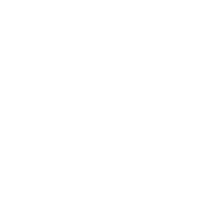
\includegraphics[max width=\textwidth]{calculations/0.png}
  \caption{Type figure caption here}
  \label{fig:0}
 \end{center}
\end{figure}
%%%
\colorbox[HTML]{808000}{\textcolor[HTML]{FFFF80}{Курсовая работа: редуктор с электродвигателем}}\newline
%%%
\colorbox[HTML]{000000}{\textcolor[HTML]{FFFF80}{\textbf{Потапов Антон R3325}}}\newline
%%%
\colorbox[HTML]{000000}{\textbf{Дано: }}\newline
%%%
\colorbox[HTML]{000000}{Вид компоновки:}\newline
%%%
\colorbox[HTML]{000000}{S1 - на одной плате, перпендикулярной оси двигателя;}\newline
%%%
\colorbox[HTML]{000000}{Условие определения числа ступеней:}\newline
%%%
\colorbox[HTML]{000000}{K1 - минимизация приведенного момента инерции;}\newline
%%%
\colorbox[HTML]{000000}{На выходном валу располагается предохранительная фрикционная муфта}\newline
%%%
\colorbox[HTML]{000000}{На выходе располагается двухпальцевый поводок.}\newline
%%%
\colorbox[HTML]{000000}{\textbf{1. Выбор электродвигателя:}}\newline
%%%
\colorbox[HTML]{000000}{Число оборотов выходного вала:}\newline
%%%
\begin{equation*}
n_{v} \defeq 145 \: \mathrm{min}^{ \operatorname{-} 1} = {2.4167 \: \mathrm{Hz}}
\end{equation*}
%%%
\colorbox[HTML]{000000}{Угловая скорость вращения выходного вала:}\newline
%%%
\begin{equation*}
ω_{v} \defeq 2 \cdot {\pi} \cdot n_{v} = {15.1844 \: \mathrm{Hz}}
\end{equation*}
%%%
\colorbox[HTML]{000000}{Момент нагрузки статический:}\newline
%%%
\begin{equation*}
M_{HC} \defeq 35 \: \mathrm{N} \: \mathrm{cm} = {0.35 \: \mathrm{J}}
\end{equation*}
%%%
\colorbox[HTML]{000000}{Момент инерции нагрузки:}\newline
%%%
\begin{equation*}
J_{H} \defeq 0.2 \: \mathrm{kg} \: \mathrm{cm}^{2} = {2 \cdot 10^{ \operatorname{-} 5} \: \mathrm{kg} \: \mathrm{m}^{2}}
\end{equation*}
%%%
\colorbox[HTML]{000000}{Угловое ускорение:}\newline
%%%
\begin{equation*}
ε_{v} \defeq 250 \: \mathrm{s}^{ \operatorname{-} 2}
\end{equation*}
%%%
\colorbox[HTML]{000000}{Динамический момент нагрузки:}\newline
%%%
\begin{equation*}
M_{HD} \defeq J_{H} \cdot ε_{v} = {0.005 \: \mathrm{J}}
\end{equation*}
%%%
\colorbox[HTML]{000000}{Статическая мощность}\newline
%%%
\begin{equation*}
N_{HC} \defeq M_{HC} \cdot ω_{v} = {5.3145 \: \mathrm{W}}
\end{equation*}
%%%
\colorbox[HTML]{000000}{Динамическая мощность}\newline
%%%
\begin{equation*}
N_{HD} \defeq M_{HD} \cdot ω_{v} = {0.0759 \: \mathrm{W}}
\end{equation*}
%%%
\colorbox[HTML]{000000}{Суммарная нагрузка на выходе механизма:}\newline
%%%
\begin{equation*}
N_{HS} \defeq N_{HC}+N_{HD} = {5.3904 \: \mathrm{W}}
\end{equation*}
%%%
\colorbox[HTML]{000000}{Коэффициент запаса:}\newline
%%%
\begin{equation*}
k \defeq 2
\end{equation*}
%%%
\colorbox[HTML]{000000}{Мощность двигателя:}\newline
%%%
\begin{equation*}
N_{DV} \defeq k \cdot N_{HS} = {10.7809 \: \mathrm{W}}
\end{equation*}
%%%
\colorbox[HTML]{000000}{\textbf{Двигатель:}}\newline
%%%
\begin{equation*}
ДПР-72-\textit{Ф2}-03
\end{equation*}
%%%
\colorbox[HTML]{000000}{Ссылка на сайт производителя:}\newline
%%%
\colorbox[HTML]{000000}{Полезная  мощность:}\newline
%%%
\colorbox[HTML]{000000}{https://eandc.ru/catalog/index.php?SECTION\_ID=227\&ELEMENT\_ID=18585}\newline
%%%
\begin{equation*}
N_{DV} \defeq 18.5 \: \mathrm{W}
\end{equation*}
%%%
\colorbox[HTML]{000000}{Частота вращения вала двигателя:}\newline
%%%
\colorbox[HTML]{000000}{Пусковой момент:}\newline
%%%
\begin{equation*}
n_{DV} \defeq 4500 \: \mathrm{min}^{ \operatorname{-} 1}
\end{equation*}
%%%
\begin{equation*}
M_{P} \defeq 245 \: \mathrm{N} \: \mathrm{mm} = {0.245 \: \mathrm{J}}
\end{equation*}
%%%
\colorbox[HTML]{000000}{Номинальный момент:}\newline
%%%
\colorbox[HTML]{000000}{Гарантийная наработка:}\newline
%%%
\begin{equation*}
M_{DV} \defeq 39.2 \: \mathrm{N} \: \mathrm{mm} = {0.0392 \: \mathrm{J}}
\end{equation*}
%%%
\begin{equation*}
L_{DV} \defeq 1000 \: \mathrm{hr}
\end{equation*}
%%%
\colorbox[HTML]{000000}{Момент инерции ротора:}\newline
%%%
\colorbox[HTML]{000000}{Масса: }\newline
%%%
\begin{equation*}
J \defeq 0.00869 \: \mathrm{kg} \: \mathrm{cm}^{2}
\end{equation*}
%%%
\begin{equation*}
mass \defeq 0.6 \: \mathrm{kg}
\end{equation*}
%%%
\colorbox[HTML]{000000}{\textbf{2. Кинематический расчет редуктора:}}\newline
%%%
\begin{equation*}
i_{MR} \defeq \frac{n_{DV}}{n_{v}} = {31.0345}
\end{equation*}
%%%
\colorbox[HTML]{000000}{Передаточные числа ступеней:}\newline
%%%
\begin{equation*}
\textit{i}_{\textit{12}} \defeq 1.6
\end{equation*}
%%%
\begin{equation*}
n_{opt} \defeq 3 \cdot \operatorname{log10} \left( i_{MR} \right) = {4.4755}
\end{equation*}
%%%
\begin{equation*}
\textit{i}_{\textit{34}} \defeq 1.85
\end{equation*}
%%%
\begin{equation*}
n \defeq 4
\end{equation*}
%%%
\begin{equation*}
\textit{i}_{\textit{56}} \defeq 2.7
\end{equation*}
%%%
\begin{equation*}
\textit{i}_{\textit{78}} \defeq 3.9 = {3.9}
\end{equation*}
%%%
\colorbox[HTML]{000000}{Числа зубьев шестерен и колес:}\newline
%%%
\begin{equation*}
\textit{Z}_{\textit{1}} \defeq 16
\end{equation*}
%%%
\begin{equation*}
\textit{Z}_{\textit{3}} \defeq \textit{Z}_{\textit{1}} = {16}
\end{equation*}
%%%
\begin{equation*}
\textit{Z}_{\textit{5}} \defeq \textit{Z}_{\textit{1}} = {16}
\end{equation*}
%%%
\begin{equation*}
\textit{Z}_{\textit{7}} \defeq \textit{Z}_{\textit{1}} = {16}
\end{equation*}
%%%
\begin{equation*}
\textit{Z}_{\textit{9}} \defeq \textit{Z}_{\textit{1}} = {16}
\end{equation*}
%%%
\begin{equation*}
\textit{Z}_{\textit{2}} \defeq \textit{Z}_{\textit{1}} \cdot \textit{i}_{\textit{12}} = {25.6}
\end{equation*}
%%%
\begin{equation*}
\textit{Z}_{\textit{2}} \defeq 26
\end{equation*}
%%%
\begin{equation*}
\textit{Z}_{\textit{4}} \defeq \textit{Z}_{\textit{3}} \cdot \textit{i}_{\textit{34}} = {29.6}
\end{equation*}
%%%
\begin{equation*}
\textit{Z}_{\textit{4}} \defeq 30
\end{equation*}
%%%
\begin{equation*}
\textit{Z}_{\textit{6}} \defeq \textit{Z}_{\textit{5}} \cdot \textit{i}_{\textit{56}} = {43.2}
\end{equation*}
%%%
\begin{equation*}
\textit{Z}_{\textit{6}} \defeq 44
\end{equation*}
%%%
\begin{equation*}
\textit{Z}_{\textit{8}} \defeq \textit{Z}_{\textit{7}} \cdot \textit{i}_{\textit{78}} = {62.4}
\end{equation*}
%%%
\begin{equation*}
\textit{Z}_{\textit{8}} \defeq 63
\end{equation*}
%%%
\colorbox[HTML]{000000}{Действительные передаточные отношения каждой пары:}\newline
%%%
\begin{equation*}
\textit{i}_{\textit{12}} \defeq \frac{\textit{Z}_{\textit{2}}}{\textit{Z}_{\textit{1}}} = {1.625}
\end{equation*}
%%%
\begin{equation*}
\textit{i}_{\textit{34}} \defeq \frac{\textit{Z}_{\textit{4}}}{\textit{Z}_{\textit{3}}} = {1.875}
\end{equation*}
%%%
\begin{equation*}
\textit{i}_{\textit{56}} \defeq \frac{\textit{Z}_{\textit{6}}}{\textit{Z}_{\textit{5}}} = {2.75}
\end{equation*}
%%%
\begin{equation*}
\textit{i}_{\textit{78}} \defeq \frac{\textit{Z}_{\textit{8}}}{\textit{Z}_{\textit{7}}} = {3.9375}
\end{equation*}
%%%
\colorbox[HTML]{000000}{Действительное передаточное \newline
отношение механизма:}\newline
%%%
\colorbox[HTML]{000000}{Расчетное значение скорости выходного вала:}\newline
%%%
\begin{equation*}
i_{MD} \defeq \textit{i}_{\textit{12}} \cdot \textit{i}_{\textit{34}} \cdot \textit{i}_{\textit{56}} \cdot \textit{i}_{\textit{78}} = {32.9919}
\end{equation*}
%%%
\begin{equation*}
n_{RV} \defeq \frac{n_{DV}}{i_{MD}} = {2.2733 \: \mathrm{Hz}}
\end{equation*}
%%%
\begin{equation*}
Δi_{MD} \defeq i_{MR}-i_{MD} = { \operatorname{-} 1.9575}
\end{equation*}
%%%
\colorbox[HTML]{FFFF80}{Условие выполняется!}\newline
%%%
\colorbox[HTML]{000000}{\textbf{3. Проектировочный расчет модуля зацепления:}}\newline
%%%
\colorbox[HTML]{000000}{Исходные данные из проектировочного расчета пятого семестра:}\newline
%%%
\colorbox[HTML]{000000}{Допускаемый угол закручивания \newline
вала на единицу длины:}\newline
%%%
\colorbox[HTML]{000000}{Для ЗК используется материал СТАЛЬ 15Х}\newline
%%%
\begin{equation*}
θ_{d} \defeq \frac{1}{10000} \: \frac{\mathrm{rad}}{\mathrm{mm}} = {0.1 \cdot \frac{1}{\mathrm{m}}}
\end{equation*}
%%%
\colorbox[HTML]{000000}{Допускаемая стрела изгиба на единицу длины вала:}\newline
%%%
\colorbox[HTML]{000000}{Термообработка:}\newline
%%%
\colorbox[HTML]{000000}{объемная закалка}\newline
%%%
\begin{equation*}
Δf \defeq \frac{1.4}{1000} = {0.0014}
\end{equation*}
%%%
\colorbox[HTML]{000000}{Коэффициент запаса прочности материала вала:}\newline
%%%
\begin{equation*}
\textit{S}_{\textit{1}} \defeq 6
\end{equation*}
%%%
\colorbox[HTML]{000000}{Вариант марки материала вала:}\newline
%%%
\colorbox[HTML]{000000}{Механические характеристики:}\newline
%%%
\begin{equation*}
\textit{k}_{\textit{1}} \defeq 3
\end{equation*}
%%%
\begin{equation*}
σ_{B} \defeq 685 \: \mathrm{MPa}
\end{equation*}
%%%
\colorbox[HTML]{000000}{Предел текучести:}\newline
%%%
\begin{equation*}
σ_{Tshaft} \defeq 320 \: \mathrm{MPa}
\end{equation*}
%%%
\begin{equation*}
σ_{T} \defeq 490 \: \mathrm{MPa}
\end{equation*}
%%%
\begin{equation*}
σ_{Bshaft} \defeq 530 \: \mathrm{MPa}
\end{equation*}
%%%
\colorbox[HTML]{000000}{Твердость }\newline
%%%
\begin{equation*}
HB_{shaft} \defeq 165
\end{equation*}
%%%
\begin{equation*}
HB \defeq 179
\end{equation*}
%%%
\colorbox[HTML]{000000}{Вариант марки материала ЗК:}\newline
%%%
\colorbox[HTML]{000000}{Долговечность работы зубчатой передачи:}\newline
%%%
\begin{equation*}
\textit{k}_{\textit{2}} \defeq 9
\end{equation*}
%%%
\begin{equation*}
L_{h} \defeq 6000 \: \mathrm{hr} = {2.16 \cdot 10^{7} \: \mathrm{s}}
\end{equation*}
%%%
\colorbox[HTML]{000000}{Степень точности и вид сопряжения ЗК:}\newline
%%%
\begin{equation*}
6-E
\end{equation*}
%%%
\colorbox[HTML]{000000}{\textbf{Расчет }}\newline
%%%
\colorbox[HTML]{000000}{Так как по условию твердость материала ЗК HB=179$<$350, габариты \newline
эвольвентной передачи определяются только контактной прочностью зубьев.}\newline
%%%
\colorbox[HTML]{000000}{Предел контактной выносливости при объемной закалке:}\newline
%%%
\begin{equation*}
σ_{HlimB} \defeq 17 \cdot H_{HRCЭ}+200
\end{equation*}
%%%
\begin{equation*}
σ_{HlimB} \defeq 17 \cdot 15 \: \mathrm{MPa}+200 \: \mathrm{MPa} = {4.55 \cdot 10^{8} \: \mathrm{Pa}}
\end{equation*}
%%%
\colorbox[HTML]{000000}{Допускаемое контактное напряжение:}\newline
%%%
\begin{equation*}
S_{H} \defeq 1.1
\end{equation*}
%%%
\begin{equation*}
Z_{N} \defeq 1
\end{equation*}
%%%
\begin{equation*}
σ_{HP} \defeq 0.9 \cdot \frac{σ_{HlimB}}{S_{H}} \cdot Z_{N} = {3.7227 \cdot 10^{8} \: \mathrm{Pa}}
\end{equation*}
%%%
\begin{figure}[h!]
 \begin{center}
  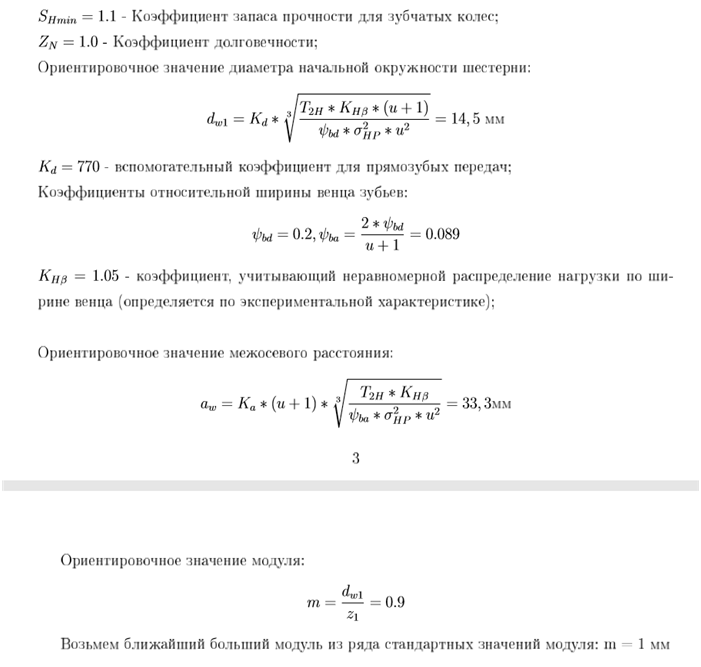
\includegraphics[max width=\textwidth]{calculations/122.png}
  \caption{Type figure caption here}
  \label{fig:122}
 \end{center}
\end{figure}
%%%
\colorbox[HTML]{000000}{Модуль :}\newline
%%%
\begin{equation*}
m \defeq 1
\end{equation*}
%%%
\colorbox[HTML]{000000}{\textbf{4. Геометрический расчет зубчатой передачи}}\newline
%%%
\colorbox[HTML]{000000}{Число зубьев:}\newline
%%%
\begin{equation*}
\textit{Z}_{\textit{1}} \defeq 16
\end{equation*}
%%%
\begin{equation*}
\textit{Z}_{\textit{3}} \defeq \textit{Z}_{\textit{1}} = {16}
\end{equation*}
%%%
\begin{equation*}
\textit{Z}_{\textit{5}} \defeq \textit{Z}_{\textit{1}} = {16}
\end{equation*}
%%%
\begin{equation*}
\textit{Z}_{\textit{7}} \defeq \textit{Z}_{\textit{1}} = {16}
\end{equation*}
%%%
\begin{equation*}
\textit{Z}_{\textit{2}} \defeq \textit{Z}_{\textit{1}} \cdot \textit{i}_{\textit{12}} = {26}
\end{equation*}
%%%
\begin{equation*}
\textit{Z}_{\textit{2}} \defeq 26
\end{equation*}
%%%
\begin{equation*}
\textit{Z}_{\textit{4}} \defeq \textit{Z}_{\textit{3}} \cdot \textit{i}_{\textit{34}} = {30}
\end{equation*}
%%%
\begin{equation*}
\textit{Z}_{\textit{4}} \defeq 30
\end{equation*}
%%%
\begin{equation*}
\textit{Z}_{\textit{6}} \defeq \textit{Z}_{\textit{5}} \cdot \textit{i}_{\textit{56}} = {44}
\end{equation*}
%%%
\begin{equation*}
\textit{Z}_{\textit{6}} \defeq 44
\end{equation*}
%%%
\begin{equation*}
\textit{Z}_{\textit{8}} \defeq \textit{Z}_{\textit{7}} \cdot \textit{i}_{\textit{78}} = {63}
\end{equation*}
%%%
\begin{equation*}
\textit{Z}_{\textit{8}} \defeq 63
\end{equation*}
%%%
\colorbox[HTML]{000000}{Модуль расчетный:}\newline
%%%
\begin{equation*}
m \defeq 1 \: \mathrm{mm}
\end{equation*}
%%%
\colorbox[HTML]{000000}{Угол наклона зубьев:}\newline
%%%
\begin{equation*}
{\beta} \defeq 0
\end{equation*}
%%%
\colorbox[HTML]{000000}{Угол профиля:}\newline
%%%
\begin{equation*}
{\alpha} \defeq 20 \: \mathrm{°}
\end{equation*}
%%%
\colorbox[HTML]{000000}{Коэффициент высоты головки:}\newline
%%%
\begin{equation*}
h_{az} \defeq 1.0
\end{equation*}
%%%
\colorbox[HTML]{000000}{Коэффициент ражиального зазора:}\newline
%%%
\begin{equation*}
c_{z} \defeq 0.25
\end{equation*}
%%%
\colorbox[HTML]{000000}{Коэффициент граничной высоты:}\newline
%%%
\begin{equation*}
h_{iz} \defeq 2
\end{equation*}
%%%
\colorbox[HTML]{000000}{Передаточное число:}\newline
%%%
\colorbox[HTML]{000000}{Действительные передаточные \newline
отношения каждой пары:}\newline
%%%
\colorbox[HTML]{000000}{Диаметры делительных окружностей:}\newline
%%%
\begin{equation*}
\textit{d}_{\textit{1}} \defeq m \cdot \textit{Z}_{\textit{1}} = {0.016 \: \mathrm{m}}
\end{equation*}
%%%
\begin{equation*}
\textit{i}_{\textit{12}} \defeq \frac{\textit{Z}_{\textit{2}}}{\textit{Z}_{\textit{1}}} = {1.625}
\end{equation*}
%%%
\begin{equation*}
\textit{d}_{\textit{2}} \defeq m \cdot \textit{Z}_{\textit{2}} = {0.026 \: \mathrm{m}}
\end{equation*}
%%%
\begin{equation*}
\textit{i}_{\textit{34}} \defeq \frac{\textit{Z}_{\textit{4}}}{\textit{Z}_{\textit{3}}} = {1.875}
\end{equation*}
%%%
\begin{equation*}
\textit{d}_{\textit{3}} \defeq m \cdot \textit{Z}_{\textit{3}} = {0.016 \: \mathrm{m}}
\end{equation*}
%%%
\begin{equation*}
\textit{i}_{\textit{56}} \defeq \frac{\textit{Z}_{\textit{6}}}{\textit{Z}_{\textit{5}}} = {2.75}
\end{equation*}
%%%
\begin{equation*}
\textit{d}_{\textit{4}} \defeq m \cdot \textit{Z}_{\textit{4}} = {0.03 \: \mathrm{m}}
\end{equation*}
%%%
\begin{equation*}
\textit{d}_{\textit{5}} \defeq m \cdot \textit{Z}_{\textit{5}} = {0.016 \: \mathrm{m}}
\end{equation*}
%%%
\begin{equation*}
\textit{i}_{\textit{78}} \defeq \frac{\textit{Z}_{\textit{8}}}{\textit{Z}_{\textit{7}}} = {3.9375}
\end{equation*}
%%%
\begin{equation*}
\textit{d}_{\textit{6}} \defeq m \cdot \textit{Z}_{\textit{6}} = {0.044 \: \mathrm{m}}
\end{equation*}
%%%
\begin{equation*}
\textit{d}_{\textit{7}} \defeq m \cdot \textit{Z}_{\textit{7}} = {0.016 \: \mathrm{m}}
\end{equation*}
%%%
\colorbox[HTML]{000000}{Угол профиля торцовый:}\newline
%%%
\begin{equation*}
\textit{d}_{\textit{8}} \defeq m \cdot \textit{Z}_{\textit{8}} = {0.063 \: \mathrm{m}}
\end{equation*}
%%%
\begin{equation*}
α_{t} \defeq 20 \: \mathrm{°}
\end{equation*}
%%%
\colorbox[HTML]{000000}{Коэффициент минимального смещения:}\newline
%%%
\begin{equation*}
\textit{x}_{\textit{min1}} \defeq h_{iz}-h_{az}-\frac{\textit{Z}_{\textit{1}} \cdot \sin \left( α_{t} \right)^{2}}{2 \cdot \cos \left( {\beta} \right)} = {0.0642}
\end{equation*}
%%%
\begin{equation*}
\textit{x}_{\textit{min2}} \defeq h_{iz}-h_{az}-\frac{\textit{Z}_{\textit{2}} \cdot \left( \sin \left( α_{t} \right) \right)^{2}}{2 \cdot \cos \left( {\beta} \right)} = { \operatorname{-} 0.5207}
\end{equation*}
%%%
\begin{equation*}
\textit{x}_{\textit{min3}} \defeq h_{iz}-h_{az}-\frac{\textit{Z}_{\textit{3}} \cdot \sin \left( α_{t} \right)^{2}}{2 \cdot \cos \left( {\beta} \right)} = {0.0642}
\end{equation*}
%%%
\begin{equation*}
\textit{x}_{\textit{min4}} \defeq h_{iz}-h_{az}-\frac{\textit{Z}_{\textit{4}} \cdot \left( \sin \left( α_{t} \right) \right)^{2}}{2 \cdot \cos \left( {\beta} \right)} = { \operatorname{-} 0.7547}
\end{equation*}
%%%
\begin{equation*}
\textit{x}_{\textit{min5}} \defeq h_{iz}-h_{az}-\frac{\textit{Z}_{\textit{5}} \cdot \sin \left( α_{t} \right)^{2}}{2 \cdot \cos \left( {\beta} \right)} = {0.0642}
\end{equation*}
%%%
\begin{equation*}
\textit{x}_{\textit{min6}} \defeq h_{iz}-h_{az}-\frac{\textit{Z}_{\textit{6}} \cdot \left( \sin \left( α_{t} \right) \right)^{2}}{2 \cdot \cos \left( {\beta} \right)} = { \operatorname{-} 1.5735}
\end{equation*}
%%%
\begin{equation*}
\textit{x}_{\textit{min7}} \defeq h_{iz}-h_{az}-\frac{\textit{Z}_{\textit{7}} \cdot \sin \left( α_{t} \right)^{2}}{2 \cdot \cos \left( {\beta} \right)} = {0.0642}
\end{equation*}
%%%
\begin{equation*}
\textit{x}_{\textit{min8}} \defeq h_{iz}-h_{az}-\frac{\textit{Z}_{\textit{8}} \cdot \left( \sin \left( α_{t} \right) \right)^{2}}{2 \cdot \cos \left( {\beta} \right)} = { \operatorname{-} 2.6848}
\end{equation*}
%%%
\colorbox[HTML]{000000}{Коэффициент смещения:}\newline
%%%
\begin{equation*}
\textit{x}_{\textit{1}} \defeq 0.07
\end{equation*}
%%%
\begin{equation*}
\textit{x}_{\textit{2}} \defeq  \operatorname{-} \textit{x}_{\textit{1}} = { \operatorname{-} 0.07}
\end{equation*}
%%%
\begin{equation*}
\textit{x}_{\textit{3}} \defeq \textit{x}_{\textit{1}} = {0.07}
\end{equation*}
%%%
\begin{equation*}
\textit{x}_{\textit{4}} \defeq  \operatorname{-} \textit{x}_{\textit{3}} = { \operatorname{-} 0.07}
\end{equation*}
%%%
\begin{equation*}
\textit{x}_{\textit{5}} \defeq \textit{x}_{\textit{1}} = {0.07}
\end{equation*}
%%%
\begin{equation*}
\textit{x}_{\textit{6}} \defeq  \operatorname{-} \textit{x}_{\textit{5}} = { \operatorname{-} 0.07}
\end{equation*}
%%%
\begin{equation*}
\textit{x}_{\textit{7}} \defeq \textit{x}_{\textit{1}} = {0.07}
\end{equation*}
%%%
\begin{equation*}
\textit{x}_{\textit{8}} \defeq  \operatorname{-} \textit{x}_{\textit{7}} = { \operatorname{-} 0.07}
\end{equation*}
%%%
\colorbox[HTML]{000000}{Угол зацепления:}\newline
%%%
\begin{equation*}
α_{tw} \defeq \operatorname{arcinv} \left( \operatorname{inv} \left( α_{t} \right)+2 \cdot \frac{\left( \textit{x}_{\textit{1}}+\textit{x}_{\textit{2}} \right)}{\textit{Z}_{\textit{1}}+\textit{Z}_{\textit{2}}} \right)
\end{equation*}
%%%
\begin{equation*}
α_{tw} \defeq 20 \: \mathrm{°}
\end{equation*}
%%%
\colorbox[HTML]{000000}{Межосевое расстояние делительное:}\newline
%%%
\begin{equation*}
\textit{a}_{\textit{12}} \defeq \frac{m \cdot \left( \textit{Z}_{\textit{1}}+\textit{Z}_{\textit{2}} \right)}{2 \cdot \cos \left( {\beta} \right)} = {0.021 \: \mathrm{m}}
\end{equation*}
%%%
\begin{equation*}
\textit{a}_{\textit{34}} \defeq \frac{m \cdot \left( \textit{Z}_{\textit{3}}+\textit{Z}_{\textit{4}} \right)}{2 \cdot \cos \left( {\beta} \right)} = {0.023 \: \mathrm{m}}
\end{equation*}
%%%
\begin{equation*}
\textit{a}_{\textit{56}} \defeq \frac{m \cdot \left( \textit{Z}_{\textit{5}}+\textit{Z}_{\textit{6}} \right)}{2 \cdot \cos \left( {\beta} \right)} = {0.03 \: \mathrm{m}}
\end{equation*}
%%%
\begin{equation*}
\textit{a}_{\textit{78}} \defeq \frac{m \cdot \left( \textit{Z}_{\textit{7}}+\textit{Z}_{\textit{8}} \right)}{2 \cdot \cos \left( {\beta} \right)} = {0.0395 \: \mathrm{m}}
\end{equation*}
%%%
\colorbox[HTML]{000000}{Межосевое расстояние:}\newline
%%%
\begin{equation*}
\textit{a}_{\textit{w12}} \defeq \textit{a}_{\textit{12}} \cdot \frac{\cos \left( α_{t} \right)}{\cos \left( α_{tw} \right)} = {0.021 \: \mathrm{m}}
\end{equation*}
%%%
\begin{equation*}
\textit{a}_{\textit{w34}} \defeq \textit{a}_{\textit{34}} \cdot \frac{\cos \left( α_{t} \right)}{\cos \left( α_{tw} \right)} = {0.023 \: \mathrm{m}}
\end{equation*}
%%%
\begin{equation*}
\textit{a}_{\textit{w56}} \defeq \textit{a}_{\textit{56}} \cdot \frac{\cos \left( α_{t} \right)}{\cos \left( α_{tw} \right)} = {0.03 \: \mathrm{m}}
\end{equation*}
%%%
\begin{equation*}
\textit{a}_{\textit{w78}} \defeq \textit{a}_{\textit{78}} \cdot \frac{\cos \left( α_{t} \right)}{\cos \left( α_{tw} \right)} = {0.0395 \: \mathrm{m}}
\end{equation*}
%%%
\colorbox[HTML]{000000}{Высота ножки зуба:}\newline
%%%
\begin{equation*}
\textit{h}_{\textit{f1}} \defeq m \cdot \left( h_{az}+c_{z}-\textit{x}_{\textit{1}} \right) = {0.0012 \: \mathrm{m}}
\end{equation*}
%%%
\begin{equation*}
\textit{h}_{\textit{f2}} \defeq m \cdot \left( h_{az}+c_{z}-\textit{x}_{\textit{2}} \right) = {0.0013 \: \mathrm{m}}
\end{equation*}
%%%
\begin{equation*}
\textit{h}_{\textit{f3}} \defeq m \cdot \left( h_{az}+c_{z}-\textit{x}_{\textit{3}} \right) = {0.0012 \: \mathrm{m}}
\end{equation*}
%%%
\begin{equation*}
\textit{h}_{\textit{f4}} \defeq m \cdot \left( h_{az}+c_{z}-\textit{x}_{\textit{4}} \right) = {0.0013 \: \mathrm{m}}
\end{equation*}
%%%
\begin{equation*}
\textit{h}_{\textit{f5}} \defeq m \cdot \left( h_{az}+c_{z}-\textit{x}_{\textit{5}} \right) = {0.0012 \: \mathrm{m}}
\end{equation*}
%%%
\begin{equation*}
\textit{h}_{\textit{f6}} \defeq m \cdot \left( h_{az}+c_{z}-\textit{x}_{\textit{6}} \right) = {0.0013 \: \mathrm{m}}
\end{equation*}
%%%
\begin{equation*}
\textit{h}_{\textit{f7}} \defeq m \cdot \left( h_{az}+c_{z}-\textit{x}_{\textit{7}} \right) = {0.0012 \: \mathrm{m}}
\end{equation*}
%%%
\begin{equation*}
\textit{h}_{\textit{f8}} \defeq m \cdot \left( h_{az}+c_{z}-\textit{x}_{\textit{8}} \right) = {0.0013 \: \mathrm{m}}
\end{equation*}
%%%
\colorbox[HTML]{000000}{Коэффициент воспринимаемого смещения:}\newline
%%%
\begin{equation*}
y \defeq \frac{a_{w}-a}{m}
\end{equation*}
%%%
\begin{equation*}
y \defeq 0
\end{equation*}
%%%
\colorbox[HTML]{000000}{Коэффициент уравнительного смещения:}\newline
%%%
\begin{equation*}
Δy \defeq \textit{x}_{\textit{1}}+\textit{x}_{\textit{2}}-y
\end{equation*}
%%%
\begin{equation*}
Δy \defeq 0
\end{equation*}
%%%
\colorbox[HTML]{000000}{Высота головки зуба:}\newline
%%%
\begin{equation*}
\textit{h}_{\textit{a1}} \defeq m \cdot \left( h_{az}+\textit{x}_{\textit{1}}-Δy \right) = {0.0011 \: \mathrm{m}}
\end{equation*}
%%%
\begin{equation*}
\textit{h}_{\textit{a2}} \defeq m \cdot \left( h_{az}+\textit{x}_{\textit{2}}-Δy \right) = {0.0009 \: \mathrm{m}}
\end{equation*}
%%%
\begin{equation*}
\textit{h}_{\textit{a3}} \defeq m \cdot \left( h_{az}+\textit{x}_{\textit{3}}-Δy \right) = {0.0011 \: \mathrm{m}}
\end{equation*}
%%%
\begin{equation*}
\textit{h}_{\textit{a4}} \defeq m \cdot \left( h_{az}+\textit{x}_{\textit{4}}-Δy \right) = {0.0009 \: \mathrm{m}}
\end{equation*}
%%%
\begin{equation*}
\textit{h}_{\textit{a5}} \defeq m \cdot \left( h_{az}+\textit{x}_{\textit{5}}-Δy \right) = {0.0011 \: \mathrm{m}}
\end{equation*}
%%%
\begin{equation*}
\textit{h}_{\textit{a6}} \defeq m \cdot \left( h_{az}+\textit{x}_{\textit{6}}-Δy \right) = {0.0009 \: \mathrm{m}}
\end{equation*}
%%%
\begin{equation*}
\textit{h}_{\textit{a7}} \defeq m \cdot \left( h_{az}+\textit{x}_{\textit{7}}-Δy \right) = {0.0011 \: \mathrm{m}}
\end{equation*}
%%%
\begin{equation*}
\textit{h}_{\textit{a8}} \defeq m \cdot \left( h_{az}+\textit{x}_{\textit{8}}-Δy \right) = {0.0009 \: \mathrm{m}}
\end{equation*}
%%%
\colorbox[HTML]{000000}{Диаметр окружности впадин:}\newline
%%%
\begin{equation*}
\textit{d}_{\textit{f1}} \defeq \textit{d}_{\textit{1}}-2 \cdot \textit{h}_{\textit{f1}} = {0.0136 \: \mathrm{m}}
\end{equation*}
%%%
\begin{equation*}
\textit{d}_{\textit{f2}} \defeq \textit{d}_{\textit{2}}-2 \cdot \textit{h}_{\textit{f2}} = {0.0234 \: \mathrm{m}}
\end{equation*}
%%%
\begin{equation*}
\textit{d}_{\textit{f3}} \defeq \textit{d}_{\textit{3}}-2 \cdot \textit{h}_{\textit{f3}} = {0.0136 \: \mathrm{m}}
\end{equation*}
%%%
\begin{equation*}
\textit{d}_{\textit{f4}} \defeq \textit{d}_{\textit{4}}-2 \cdot \textit{h}_{\textit{f4}} = {0.0274 \: \mathrm{m}}
\end{equation*}
%%%
\colorbox[HTML]{000000}{Диаметр окружности вершин:}\newline
%%%
\begin{equation*}
\textit{d}_{\textit{f5}} \defeq \textit{d}_{\textit{5}}-2 \cdot \textit{h}_{\textit{f5}} = {0.0136 \: \mathrm{m}}
\end{equation*}
%%%
\begin{equation*}
\textit{d}_{\textit{a1}} \defeq \textit{d}_{\textit{1}}+2 \cdot \textit{h}_{\textit{a1}} = {0.0181 \: \mathrm{m}}
\end{equation*}
%%%
\begin{equation*}
\textit{d}_{\textit{f6}} \defeq \textit{d}_{\textit{6}}-2 \cdot \textit{h}_{\textit{f6}} = {0.0414 \: \mathrm{m}}
\end{equation*}
%%%
\begin{equation*}
\textit{d}_{\textit{f7}} \defeq \textit{d}_{\textit{7}}-2 \cdot \textit{h}_{\textit{f7}} = {0.0136 \: \mathrm{m}}
\end{equation*}
%%%
\begin{equation*}
\textit{d}_{\textit{a2}} \defeq \textit{d}_{\textit{2}}+2 \cdot \textit{h}_{\textit{a2}} = {0.0279 \: \mathrm{m}}
\end{equation*}
%%%
\begin{equation*}
\textit{d}_{\textit{f8}} \defeq \textit{d}_{\textit{8}}-2 \cdot \textit{h}_{\textit{f8}} = {0.0604 \: \mathrm{m}}
\end{equation*}
%%%
\begin{equation*}
\textit{d}_{\textit{a3}} \defeq \textit{d}_{\textit{3}}+2 \cdot \textit{h}_{\textit{a3}} = {0.0181 \: \mathrm{m}}
\end{equation*}
%%%
\begin{equation*}
\textit{d}_{\textit{a4}} \defeq \textit{d}_{\textit{4}}+2 \cdot \textit{h}_{\textit{a4}} = {0.0319 \: \mathrm{m}}
\end{equation*}
%%%
\begin{equation*}
\textit{d}_{\textit{a5}} \defeq \textit{d}_{\textit{5}}+2 \cdot \textit{h}_{\textit{a5}} = {0.0181 \: \mathrm{m}}
\end{equation*}
%%%
\begin{equation*}
\textit{d}_{\textit{a6}} \defeq \textit{d}_{\textit{6}}+2 \cdot \textit{h}_{\textit{a6}} = {0.0459 \: \mathrm{m}}
\end{equation*}
%%%
\begin{equation*}
\textit{d}_{\textit{a7}} \defeq \textit{d}_{\textit{7}}+2 \cdot \textit{h}_{\textit{a7}} = {0.0181 \: \mathrm{m}}
\end{equation*}
%%%
\begin{equation*}
\textit{d}_{\textit{a8}} \defeq \textit{d}_{\textit{8}}+2 \cdot \textit{h}_{\textit{a8}} = {0.0649 \: \mathrm{m}}
\end{equation*}
%%%
\colorbox[HTML]{000000}{Минимальное число зубьев свободное от подрезания:}\newline
%%%
\begin{equation*}
\textit{z}_{\textit{min1}} \defeq 2 \cdot \left( \frac{h_{iz}-h_{az}-\textit{x}_{\textit{1}}}{\sin \left( α_{t} \right)^{2}} \right) = {15.9005}
\end{equation*}
%%%
\begin{equation*}
\textit{z}_{\textit{min2}} \defeq 2 \cdot \left( \frac{h_{iz}-h_{az}-\textit{x}_{\textit{2}}}{\sin \left( α_{t} \right)^{2}} \right) = {18.2941}
\end{equation*}
%%%
\begin{equation*}
\textit{z}_{\textit{min3}} \defeq 2 \cdot \left( \frac{h_{iz}-h_{az}-\textit{x}_{\textit{3}}}{\sin \left( α_{t} \right)^{2}} \right) = {15.9005}
\end{equation*}
%%%
\begin{equation*}
\textit{zmin4} \defeq 2 \cdot \left( \frac{h_{iz}-h_{az}-\textit{x}_{\textit{4}}}{\sin \left( α_{t} \right)^{2}} \right) = {18.2941}
\end{equation*}
%%%
\begin{equation*}
\textit{z}_{\textit{min5}} \defeq 2 \cdot \left( \frac{h_{iz}-h_{az}-\textit{x}_{\textit{5}}}{\sin \left( α_{t} \right)^{2}} \right) = {15.9005}
\end{equation*}
%%%
\begin{equation*}
\textit{z}_{\textit{min6}} \defeq 2 \cdot \left( \frac{h_{iz}-h_{az}-\textit{x}_{\textit{6}}}{\sin \left( α_{t} \right)^{2}} \right) = {18.2941}
\end{equation*}
%%%
\begin{equation*}
\textit{z}_{\textit{min7}} \defeq 2 \cdot \left( \frac{h_{iz}-h_{az}-\textit{x}_{\textit{7}}}{\sin \left( α_{t} \right)^{2}} \right) = {15.9005}
\end{equation*}
%%%
\begin{equation*}
\textit{z}_{\textit{min8}} \defeq 2 \cdot \left( \frac{h_{iz}-h_{az}-\textit{x}_{\textit{8}}}{\sin \left( α_{t} \right)^{2}} \right) = {18.2941}
\end{equation*}
%%%
\colorbox[HTML]{000000}{Диаметр измерительных роликов:}\newline
%%%
\begin{equation*}
D \defeq 1.732 \: \mathrm{mm}
\end{equation*}
%%%
\colorbox[HTML]{000000}{Угол развернутости эвольвенты в точке касания измерительных роликов:}\newline
%%%
\begin{equation*}
\operatorname{inv} \left( t \right) \defeq \tan \left( t \right)-t
\end{equation*}
%%%
\begin{equation*}
\textit{invα}_{\textit{D1}} \defeq \frac{D}{m \cdot \textit{Z}_{\textit{1}}}+\operatorname{inv} \left( α_{t} \right)-\frac{{\pi}}{2 \cdot \textit{Z}_{\textit{1}}}+\frac{2 \cdot \textit{x}_{\textit{1}}}{\textit{Z}_{\textit{1}}} \cdot \tan \left( {\alpha} \right) = {0.0282}
\end{equation*}
%%%
\begin{equation*}
\textit{invα}_{\textit{D2}} \defeq \frac{D}{m \cdot \textit{Z}_{\textit{2}}}+\operatorname{inv} \left( α_{t} \right)-\frac{{\pi}}{2 \cdot \textit{Z}_{\textit{2}}}+\frac{2 \cdot \textit{x}_{\textit{2}}}{\textit{Z}_{\textit{2}}} \cdot \tan \left( {\alpha} \right) = {0.0191}
\end{equation*}
%%%
\begin{equation*}
\textit{invα}_{\textit{D3}} \defeq \frac{D}{m \cdot \textit{Z}_{\textit{3}}}+\operatorname{inv} \left( α_{t} \right)-\frac{{\pi}}{2 \cdot \textit{Z}_{\textit{3}}}+\frac{2 \cdot \textit{x}_{\textit{3}}}{\textit{Z}_{\textit{3}}} \cdot \tan \left( {\alpha} \right) = {0.0282}
\end{equation*}
%%%
\begin{equation*}
\textit{invα}_{\textit{D4}} \defeq \frac{D}{m \cdot \textit{Z}_{\textit{4}}}+\operatorname{inv} \left( α_{t} \right)-\frac{{\pi}}{2 \cdot \textit{Z}_{\textit{4}}}+\frac{2 \cdot \textit{x}_{\textit{4}}}{\textit{Z}_{\textit{4}}} \cdot \tan \left( {\alpha} \right) = {0.0186}
\end{equation*}
%%%
\begin{equation*}
\textit{invα}_{\textit{D5}} \defeq \frac{D}{m \cdot \textit{Z}_{\textit{5}}}+\operatorname{inv} \left( α_{t} \right)-\frac{{\pi}}{2 \cdot \textit{Z}_{\textit{5}}}+\frac{2 \cdot \textit{x}_{\textit{5}}}{\textit{Z}_{\textit{5}}} \cdot \tan \left( {\alpha} \right) = {0.0282}
\end{equation*}
%%%
\begin{equation*}
\textit{invα}_{\textit{D6}} \defeq \frac{D}{m \cdot \textit{Z}_{\textit{6}}}+\operatorname{inv} \left( α_{t} \right)-\frac{{\pi}}{2 \cdot \textit{Z}_{\textit{6}}}+\frac{2 \cdot \textit{x}_{\textit{6}}}{\textit{Z}_{\textit{6}}} \cdot \tan \left( {\alpha} \right) = {0.0174}
\end{equation*}
%%%
\begin{equation*}
\textit{invα}_{\textit{D7}} \defeq \frac{D}{m \cdot \textit{Z}_{\textit{7}}}+\operatorname{inv} \left( α_{t} \right)-\frac{{\pi}}{2 \cdot \textit{Z}_{\textit{7}}}+\frac{2 \cdot \textit{x}_{\textit{7}}}{\textit{Z}_{\textit{7}}} \cdot \tan \left( {\alpha} \right) = {0.0282}
\end{equation*}
%%%
\begin{equation*}
\textit{invα}_{\textit{D8}} \defeq \frac{D}{m \cdot \textit{Z}_{\textit{8}} \cdot \cos \left( {\alpha} \right)}+\operatorname{inv} \left( α_{t} \right)-\frac{{\pi}}{2 \cdot \textit{Z}_{\textit{8}}}+\frac{2 \cdot \textit{x}_{\textit{8}}}{\textit{Z}_{\textit{8}}} \cdot \tan \left( {\alpha} \right) = {0.0184}
\end{equation*}
%%%
\begin{equation*}
\textit{α}_{\textit{D1}} \defeq 24.53 \: \mathrm{grad}
\end{equation*}
%%%
\begin{equation*}
\textit{α}_{\textit{D3}} \defeq 24.53 \: \mathrm{grad}
\end{equation*}
%%%
\begin{equation*}
\textit{α}_{\textit{D6}} \defeq 21.47 \: \mathrm{grad}
\end{equation*}
%%%
\begin{equation*}
\textit{α}_{\textit{D2}} \defeq 21.8 \: \mathrm{grad}
\end{equation*}
%%%
\begin{equation*}
\textit{α}_{\textit{D4}} \defeq 21.67 \: \mathrm{grad}
\end{equation*}
%%%
\begin{equation*}
\textit{α}_{\textit{D7}} \defeq 24.53 \: \mathrm{grad}
\end{equation*}
%%%
\begin{equation*}
\textit{α}_{\textit{D5}} \defeq 24.53 \: \mathrm{grad}
\end{equation*}
%%%
\begin{equation*}
\textit{α}_{\textit{D8}} \defeq 21.07 \: \mathrm{grad}
\end{equation*}
%%%
\colorbox[HTML]{000000}{Размер по роликам:}\newline
%%%
\begin{equation*}
\textit{M}_{\textit{1}} \defeq \frac{m \cdot \textit{Z}_{\textit{1}} \cdot \cos \left( α_{t} \right)}{\cos \left( \textit{α}_{\textit{D1}} \right)}+D = {0.018 \: \mathrm{m}}
\end{equation*}
%%%
\begin{equation*}
\textit{M}_{\textit{5}} \defeq \frac{m \cdot \textit{Z}_{\textit{5}} \cdot \cos \left( α_{t} \right)}{\cos \left( \textit{α}_{\textit{D5}} \right)}+D = {0.018 \: \mathrm{m}}
\end{equation*}
%%%
\begin{equation*}
\textit{M}_{\textit{2}} \defeq \frac{m \cdot \textit{Z}_{\textit{3}} \cdot \cos \left( α_{t} \right)}{\cos \left( \textit{α}_{\textit{D2}} \right)}+D = {0.0177 \: \mathrm{m}}
\end{equation*}
%%%
\begin{equation*}
\textit{M}_{\textit{6}} \defeq \frac{m \cdot \textit{Z}_{\textit{6}} \cdot \cos \left( α_{t} \right)}{\cos \left( \textit{α}_{\textit{D6}} \right)}+D = {0.0455 \: \mathrm{m}}
\end{equation*}
%%%
\begin{equation*}
\textit{M}_{\textit{3}} \defeq \frac{m \cdot \textit{Z}_{\textit{3}} \cdot \cos \left( α_{t} \right)}{\cos \left( \textit{α}_{\textit{D3}} \right)}+D = {0.018 \: \mathrm{m}}
\end{equation*}
%%%
\begin{equation*}
\textit{M}_{\textit{7}} \defeq \frac{m \cdot \textit{Z}_{\textit{7}} \cdot \cos \left( α_{t} \right)}{\cos \left( \textit{α}_{\textit{D7}} \right)}+D = {0.018 \: \mathrm{m}}
\end{equation*}
%%%
\begin{equation*}
\textit{M}_{\textit{4}} \defeq \frac{m \cdot \textit{Z}_{\textit{4}} \cdot \cos \left( α_{t} \right)}{\cos \left( \textit{α}_{\textit{D4}} \right)}+D = {0.0316 \: \mathrm{m}}
\end{equation*}
%%%
\begin{equation*}
\textit{M}_{\textit{8}} \defeq \frac{m \cdot \textit{Z}_{\textit{8}} \cdot \cos \left( α_{t} \right)}{\cos \left( \textit{α}_{\textit{D8}} \right)} \cdot \cos \left( \frac{{\pi}}{2 \cdot \textit{Z}_{\textit{8}}} \right)+D = {0.06431 \: \mathrm{m}}
\end{equation*}
%%%
\colorbox[HTML]{000000}{\textbf{5. Выбор показателя точности зубчатых передач }}\newline
%%%
\begin{equation*}
\textit{E}_{\textit{Ms1}} \defeq 58 \: \mathrm{μm}
\end{equation*}
%%%
\begin{equation*}
\textit{E}_{\textit{Ms2}} \defeq 70 \: \mathrm{μm}
\end{equation*}
%%%
\begin{equation*}
\textit{E}_{\textit{Ms7}} \defeq 58 \: \mathrm{μm}
\end{equation*}
%%%
\begin{equation*}
\textit{E}_{\textit{Ms8}} \defeq 85 \: \mathrm{μm}
\end{equation*}
%%%
\begin{equation*}
\textit{T}_{\textit{M1}} \defeq 32 \: \mathrm{μm}
\end{equation*}
%%%
\begin{equation*}
\textit{T}_{\textit{M2}} \defeq 36 \: \mathrm{μm}
\end{equation*}
%%%
\begin{equation*}
\textit{T}_{\textit{M7}} \defeq 32 \: \mathrm{μm}
\end{equation*}
%%%
\begin{equation*}
\textit{T}_{\textit{M8}} \defeq 40 \: \mathrm{μm}
\end{equation*}
%%%
\begin{equation*}
\textit{E}_{\textit{Ms3}} \defeq 58 \: \mathrm{μm}
\end{equation*}
%%%
\begin{equation*}
\textit{E}_{\textit{Ms4}} \defeq 70 \: \mathrm{μm}
\end{equation*}
%%%
\begin{equation*}
\textit{E}_{\textit{Ms9}} \defeq 58 \: \mathrm{μm}
\end{equation*}
%%%
\begin{equation*}
\textit{E}_{\textit{Ms10}} \defeq 100 \: \mathrm{μm}
\end{equation*}
%%%
\begin{equation*}
\textit{T}_{\textit{M3}} \defeq 32 \: \mathrm{μm}
\end{equation*}
%%%
\begin{equation*}
\textit{T}_{\textit{M4}} \defeq 36 \: \mathrm{μm}
\end{equation*}
%%%
\begin{equation*}
\textit{T}_{\textit{M9}} \defeq 32 \: \mathrm{μm}
\end{equation*}
%%%
\begin{equation*}
\textit{T}_{\textit{M10}} \defeq 48 \: \mathrm{μm}
\end{equation*}
%%%
\begin{equation*}
\textit{E}_{\textit{Ms5}} \defeq 58 \: \mathrm{μm}
\end{equation*}
%%%
\begin{equation*}
\textit{E}_{\textit{Ms6}} \defeq 70 \: \mathrm{μm}
\end{equation*}
%%%
\begin{equation*}
\textit{T}_{\textit{M5}} \defeq 32 \: \mathrm{μm}
\end{equation*}
%%%
\begin{equation*}
\textit{T}_{\textit{M6}} \defeq 36 \: \mathrm{μm}
\end{equation*}
%%%
\colorbox[HTML]{000000}{Отклонения размеров по роликам M:}\newline
%%%
\begin{equation*}
\textit{M}_{\textit{T2}} \defeq  \operatorname{-} \textit{E}_{\textit{Ms2}} = { \operatorname{-} 7 \cdot 10^{ \operatorname{-} 5} \: \mathrm{m}}
\end{equation*}
%%%
\begin{equation*}
\textit{MT1} \defeq  \operatorname{-} \textit{E}_{\textit{Ms1}} = { \operatorname{-} 5.8 \cdot 10^{ \operatorname{-} 5} \: \mathrm{m}}
\end{equation*}
%%%
\begin{equation*}
\textit{M}_{\textit{D1}} \defeq  \operatorname{-} \left( \textit{E}_{\textit{Ms1}}+\textit{T}_{\textit{M1}} \right) = { \operatorname{-} 9 \cdot 10^{ \operatorname{-} 5} \: \mathrm{m}}
\end{equation*}
%%%
\begin{equation*}
\textit{M}_{\textit{D2}} \defeq  \operatorname{-} \left( \textit{E}_{\textit{Ms2}}+\textit{T}_{\textit{M2}} \right) = { \operatorname{-} 0.000106 \: \mathrm{m}}
\end{equation*}
%%%
\begin{equation*}
\textit{M}_{\textit{T3}} \defeq  \operatorname{-} \textit{E}_{\textit{Ms3}} = { \operatorname{-} 5.8 \cdot 10^{ \operatorname{-} 5} \: \mathrm{m}}
\end{equation*}
%%%
\begin{equation*}
\textit{M}_{\textit{T4}} \defeq  \operatorname{-} \textit{E}_{\textit{Ms4}} = { \operatorname{-} 7 \cdot 10^{ \operatorname{-} 5} \: \mathrm{m}}
\end{equation*}
%%%
\begin{equation*}
\textit{M}_{\textit{D3}} \defeq  \operatorname{-} \left( \textit{E}_{\textit{Ms3}}+\textit{T}_{\textit{M3}} \right) = { \operatorname{-} 9 \cdot 10^{ \operatorname{-} 5} \: \mathrm{m}}
\end{equation*}
%%%
\begin{equation*}
\textit{M}_{\textit{D4}} \defeq  \operatorname{-} \left( \textit{E}_{\textit{Ms4}}+\textit{T}_{\textit{M4}} \right) = { \operatorname{-} 0.000106 \: \mathrm{m}}
\end{equation*}
%%%
\begin{equation*}
\textit{M}_{\textit{T5}} \defeq  \operatorname{-} \textit{E}_{\textit{Ms5}} = { \operatorname{-} 5.8 \cdot 10^{ \operatorname{-} 5} \: \mathrm{m}}
\end{equation*}
%%%
\begin{equation*}
\textit{M}_{\textit{T6}} \defeq  \operatorname{-} \textit{E}_{\textit{Ms6}} = { \operatorname{-} 7 \cdot 10^{ \operatorname{-} 5} \: \mathrm{m}}
\end{equation*}
%%%
\begin{equation*}
\textit{M}_{\textit{D5}} \defeq  \operatorname{-} \left( \textit{E}_{\textit{Ms5}}+\textit{T}_{\textit{M5}} \right) = { \operatorname{-} 9 \cdot 10^{ \operatorname{-} 5} \: \mathrm{m}}
\end{equation*}
%%%
\begin{equation*}
\textit{M}_{\textit{D6}} \defeq  \operatorname{-} \left( \textit{E}_{\textit{Ms6}}+\textit{T}_{\textit{M6}} \right) = { \operatorname{-} 0.000106 \: \mathrm{m}}
\end{equation*}
%%%
\begin{equation*}
\textit{M}_{\textit{T7}} \defeq  \operatorname{-} \textit{E}_{\textit{Ms7}} = { \operatorname{-} 5.8 \cdot 10^{ \operatorname{-} 5} \: \mathrm{m}}
\end{equation*}
%%%
\begin{equation*}
\textit{M}_{\textit{T8}} \defeq  \operatorname{-} \textit{E}_{\textit{Ms8}} = { \operatorname{-} 8.5 \cdot 10^{ \operatorname{-} 5} \: \mathrm{m}}
\end{equation*}
%%%
\begin{equation*}
\textit{M}_{\textit{D7}} \defeq  \operatorname{-} \left( \textit{E}_{\textit{Ms7}}+\textit{T}_{\textit{M7}} \right) = { \operatorname{-} 9 \cdot 10^{ \operatorname{-} 5} \: \mathrm{m}}
\end{equation*}
%%%
\begin{equation*}
\textit{M}_{\textit{D8}} \defeq  \operatorname{-} \left( \textit{E}_{\textit{Ms8}}+\textit{T}_{\textit{M8}} \right) = { \operatorname{-} 0.000125 \: \mathrm{m}}
\end{equation*}
%%%
\colorbox[HTML]{000000}{\textbf{6. Расчёт вращательных моментов на валах}}\newline
%%%
\colorbox[HTML]{000000}{Суммарный момент нагрузки:}\newline
%%%
\begin{equation*}
M_{Σ} \defeq M_{HD}+M_{HC} = {0.355 \: \mathrm{J}}
\end{equation*}
%%%
\colorbox[HTML]{000000}{Для данной схемы:}\newline
%%%
\begin{equation*}

\left| \begin{aligned}
\,&M_{V} \defeq M_{Σ}\end{aligned} \right. = {0.355 \: \mathrm{J}}
\end{equation*}
%%%
\colorbox[HTML]{000000}{Для заданной степени точности зубчатых колес \newline
коэффициент трения скольжения стальных ЗК:}\newline
%%%
\begin{equation*}
f \defeq 0.08
\end{equation*}
%%%
\colorbox[HTML]{000000}{\textbf{На IV валу:}}\newline
%%%
\colorbox[HTML]{000000}{Нормальное усилие в зацеплении:}\newline
%%%
\begin{equation*}
\textit{F}_{\textit{n78}} \defeq \frac{2 \cdot M_{V}}{m \cdot \textit{Z}_{\textit{8}} \cdot \cos \left( α_{t} \right)} = {11.9931 \: \mathrm{N}}
\end{equation*}
%%%
\colorbox[HTML]{000000}{Поправочный коэффициент:}\newline
%%%
\begin{equation*}
\textit{C}_{\textit{78}} \defeq \frac{\textit{F}_{\textit{n78}}+3 \: \mathrm{N}}{\textit{F}_{\textit{n78}}+0.2 \: \mathrm{N}} = {1.2296}
\end{equation*}
%%%
\begin{equation*}
\textit{η}_{\textit{78}} \defeq 1-\textit{C}_{\textit{78}} \cdot f \cdot {\pi} \cdot \left( \frac{1}{\textit{Z}_{\textit{8}}}+\frac{1}{\textit{Z}_{\textit{7}}} \right) = {0.9758}
\end{equation*}
%%%
\begin{equation*}
M_{IV} \defeq \frac{M_{V}}{\textit{η}_{\textit{78}} \cdot \textit{i}_{\textit{78}}} = {0.0924 \: \mathrm{J}}
\end{equation*}
%%%
\colorbox[HTML]{000000}{\textbf{На III валу:}}\newline
%%%
\colorbox[HTML]{000000}{Нормальное усилие в зацеплении:}\newline
%%%
\begin{equation*}
\textit{F}_{\textit{n65}} \defeq \frac{2 \cdot M_{IV}}{m \cdot \textit{Z}_{\textit{6}} \cdot \cos \left( α_{t} \right)} = {4.4694 \: \mathrm{N}}
\end{equation*}
%%%
\colorbox[HTML]{000000}{Поправочный коэффициент:}\newline
%%%
\begin{equation*}
\textit{C}_{\textit{65}} \defeq \frac{\textit{F}_{\textit{n65}}+3 \: \mathrm{N}}{\textit{F}_{\textit{n65}}+0.2 \: \mathrm{N}} = {1.5997}
\end{equation*}
%%%
\begin{equation*}
\textit{η}_{\textit{65}} \defeq 1-\textit{C}_{\textit{65}} \cdot f \cdot {\pi} \cdot \left( \frac{1}{\textit{Z}_{\textit{6}}}+\frac{1}{\textit{Z}_{\textit{5}}} \right) = {0.9657}
\end{equation*}
%%%
\begin{equation*}
M_{III} \defeq \frac{M_{IV}}{\textit{η}_{\textit{65}} \cdot \textit{i}_{\textit{56}}} = {0.0348 \: \mathrm{J}}
\end{equation*}
%%%
\colorbox[HTML]{000000}{\textbf{На II валу:}}\newline
%%%
\colorbox[HTML]{000000}{Нормальное усилие в зацеплении:}\newline
%%%
\begin{equation*}
\textit{F}_{\textit{n43}} \defeq \frac{2 \cdot M_{III}}{m \cdot \textit{Z}_{\textit{4}} \cdot \cos \left( α_{t} \right)} = {2.4682 \: \mathrm{N}}
\end{equation*}
%%%
\colorbox[HTML]{000000}{Поправочный коэффициент:}\newline
%%%
\begin{equation*}
\textit{C}_{\textit{43}} \defeq \frac{\textit{F}_{\textit{n43}}+3 \: \mathrm{N}}{\textit{F}_{\textit{n43}}+0.2 \: \mathrm{N}} = {2.0494}
\end{equation*}
%%%
\begin{equation*}
\textit{η}_{\textit{43}} \defeq 1-\textit{C}_{\textit{43}} \cdot f \cdot {\pi} \cdot \left( \frac{1}{\textit{Z}_{\textit{4}}}+\frac{1}{\textit{Z}_{\textit{3}}} \right) = {0.9506}
\end{equation*}
%%%
\begin{equation*}
M_{II} \defeq \frac{M_{III}}{\textit{η}_{\textit{43}} \cdot \textit{i}_{\textit{34}}} = {0.0195 \: \mathrm{J}}
\end{equation*}
%%%
\colorbox[HTML]{000000}{\textbf{На I валу:}}\newline
%%%
\colorbox[HTML]{000000}{Нормальное усилие в зацеплении:}\newline
%%%
\begin{equation*}
\textit{F}_{\textit{n21}} \defeq \frac{2 \cdot M_{II}}{m \cdot \textit{Z}_{\textit{2}} \cdot \cos \left( α_{t} \right)} = {1.5978 \: \mathrm{N}}
\end{equation*}
%%%
\colorbox[HTML]{000000}{Поправочный коэффициент:}\newline
%%%
\begin{equation*}
\textit{C}_{\textit{21}} \defeq \frac{\textit{F}_{\textit{n21}}+3 \: \mathrm{N}}{\textit{F}_{\textit{n21}}+0.2 \: \mathrm{N}} = {2.5575}
\end{equation*}
%%%
\begin{equation*}
\textit{η}_{\textit{21}} \defeq 1-\textit{C}_{\textit{21}} \cdot f \cdot {\pi} \cdot \left( \frac{1}{\textit{Z}_{\textit{2}}}+\frac{1}{\textit{Z}_{\textit{1}}} \right) = {0.9351}
\end{equation*}
%%%
\begin{equation*}
M_{I} \defeq \frac{M_{II}}{\textit{η}_{\textit{21}} \cdot \textit{i}_{\textit{12}}} = {0.0128 \: \mathrm{J}}
\end{equation*}
%%%
\colorbox[HTML]{000000}{\textbf{7. Расчет валов на статическую прочность}}\newline
%%%
\colorbox[HTML]{000000}{Механические характеристики конструкционной стали, используемой для изготовления вала}\newline
%%%
\colorbox[HTML]{000000}{Упругие константы углеродистых сталей:}\newline
%%%
\colorbox[HTML]{000000}{E = 1.95..2.05 *10$\wedge$5 МПа - модуль упругости первого рода;}\newline
%%%
\colorbox[HTML]{000000}{G = 0.80..0.81 *10$\wedge$5 МПа - модуль упругости второго рода;}\newline
%%%
\colorbox[HTML]{000000}{ν = 0.024..0.028 - коэффициент Пуассона;}\newline
%%%
\begin{equation*}
G \defeq 0.8 \cdot 10^{5} \: \mathrm{MPa} = {8 \cdot 10^{10} \: \mathrm{Pa}}
\end{equation*}
%%%
\colorbox[HTML]{000000}{Марки стали: Сталь 35;}\newline
%%%
\begin{equation*}
σ_{BV} \geq 600 \: \mathrm{MPa}
\end{equation*}
%%%
\begin{equation*}
σ_{TV} \geq 320 \: \mathrm{MPa}
\end{equation*}
%%%
\begin{equation*}
τ_{TV} \geq 190 \: \mathrm{MPa}
\end{equation*}
%%%
\begin{equation*}
\textit{σ}_{\textit{И\_1}} \defeq 220-300 \: \mathrm{MPa}
\end{equation*}
%%%
\begin{equation*}
\textit{σ}_{\textit{Р\_1}} \defeq 170-220 \: \mathrm{MPa}
\end{equation*}
%%%
\begin{equation*}
\textit{τ}_{\textit{k\_1}} \defeq 130-180 \: \mathrm{MPa}
\end{equation*}
%%%
\begin{equation*}
σ_{BV} \defeq 600 \: \mathrm{MPa}
\end{equation*}
%%%
\begin{equation*}
σ_{TV} \defeq 320 \: \mathrm{MPa}
\end{equation*}
%%%
\begin{equation*}
τ_{TV} \defeq 190 \: \mathrm{MPa}
\end{equation*}
%%%
\begin{equation*}
\textit{σ}_{\textit{И\_1}} \defeq 220-300 \: \mathrm{MPa}
\end{equation*}
%%%
\begin{equation*}
\textit{σ}_{\textit{Р\_1}} \defeq 170-220 \: \mathrm{MPa}
\end{equation*}
%%%
\begin{equation*}
\textit{τ}_{\textit{k\_1}} \defeq 130-180 \: \mathrm{MPa}
\end{equation*}
%%%
\colorbox[HTML]{000000}{Допускаемое напряжение при кручении:}\newline
%%%
\begin{equation*}
τ_{dk} \defeq \frac{σ_{TV}}{\textit{S}_{\textit{1}}} = {5.3333 \cdot 10^{7} \: \mathrm{Pa}}
\end{equation*}
%%%
\colorbox[HTML]{000000}{С учетом того, что при проектировочном расчете валов допускаемые напряжения обычно занижают:}\newline
%%%
\begin{equation*}
τ_{dk} \defeq 20 \: \mathrm{MPa}
\end{equation*}
%%%
\colorbox[HTML]{000000}{По условию статической прочности вала на кручение:}\newline
%%%
\begin{equation*}
d_{min} \defeq \left( \frac{M_{V}}{0.2 \cdot τ_{dk}} \right)^{\frac{1}{3}} = {0.0045 \: \mathrm{m}}
\end{equation*}
%%%
\colorbox[HTML]{000000}{По условию крутильной жесткости вала:}\newline
%%%
\begin{equation*}
d_{min} \defeq \left( \frac{M_{V}}{0.1 \cdot G \cdot θ_{d}} \right)^{\frac{1}{4}} = {0.0046 \: \mathrm{m}}
\end{equation*}
%%%
\begin{equation*}
dm \defeq 5 \: \mathrm{mm}
\end{equation*}
%%%
\colorbox[HTML]{000000}{Радиальная составляющая силы резания:}\newline
%%%
\begin{equation*}
P \defeq 150+\textit{S}_{\textit{1}} \cdot 10 = {210}
\end{equation*}
%%%
\colorbox[HTML]{000000}{Длина вала, округленная до ближайшего целого:}\newline
%%%
\begin{equation*}
L \defeq 10 \cdot dm = {0.05 \: \mathrm{m}}
\end{equation*}
%%%
\colorbox[HTML]{000000}{Допускаемая деформация изгиба вала:}\newline
%%%
\begin{equation*}
Δf_{ud} \defeq Δf \cdot L = {7 \cdot 10^{ \operatorname{-} 5} \: \mathrm{m}}
\end{equation*}
%%%
\colorbox[HTML]{000000}{\textbf{Модуль первого рода:}}\newline
%%%
\begin{equation*}
E \defeq 200000 \: \mathrm{MPa}
\end{equation*}
%%%
\begin{equation*}
d \defeq \left( \frac{1.3 \: \mathrm{N} \cdot P \cdot L^{3}}{E \cdot {\pi} \cdot Δf_{ud}} \right)^{\frac{1}{4}} = {0.00528 \: \mathrm{m}}
\end{equation*}
%%%
\begin{equation*}
d \defeq 0.006 \: \mathrm{m}
\end{equation*}
%%%
\colorbox[HTML]{000000}{Диаметры валов:}\newline
%%%
\begin{equation*}
d_{I} \defeq 4
\end{equation*}
%%%
\begin{equation*}
d_{II} \defeq 5
\end{equation*}
%%%
\begin{equation*}
d_{III} \defeq 5
\end{equation*}
%%%
\begin{equation*}
d_{IV} \defeq 5
\end{equation*}
%%%
\begin{equation*}
d_{V} \defeq 6
\end{equation*}
%%%
\colorbox[HTML]{000000}{\textbf{8. Выбор посадок для сопрягаемых деталей.}}\newline
%%%
\begin{figure}[h!]
 \begin{center}
  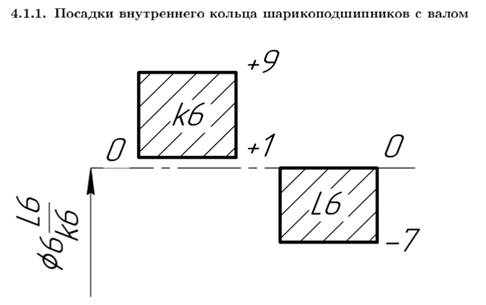
\includegraphics[max width=\textwidth]{calculations/398.png}
  \caption{Type figure caption here}
  \label{fig:398}
 \end{center}
\end{figure}
%%%
\colorbox[HTML]{000000}{Посадка вешнего кольца шарикоподшипников с подшипниковой втулкой:}\newline
%%%
\begin{figure}[h!]
 \begin{center}
  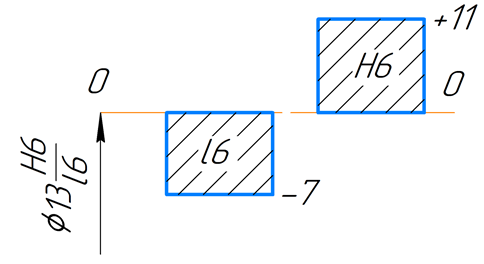
\includegraphics[max width=\textwidth]{calculations/400.png}
  \caption{Type figure caption here}
  \label{fig:400}
 \end{center}
\end{figure}
%%%
\begin{figure}[h!]
 \begin{center}
  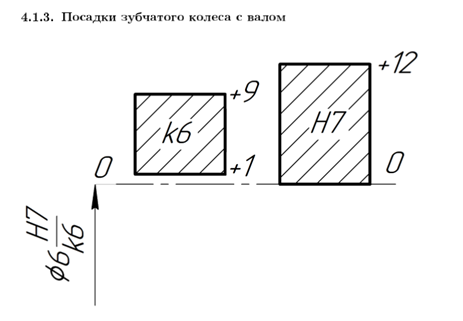
\includegraphics[max width=\textwidth]{calculations/401.png}
  \caption{Type figure caption here}
  \label{fig:401}
 \end{center}
\end{figure}
%%%
\colorbox[HTML]{000000}{\textbf{9. Проверочные расчеты:}}\newline
%%%
\colorbox[HTML]{000000}{\textbf{9.1 Расчет цилиндрической зубчатой передачи на контактную прочность /выносливость}}\newline
%%%
\colorbox[HTML]{000000}{Окружная сила на делительном цилиндре:}\newline
%%%
\begin{equation*}
F_{tH} \defeq 2 \cdot \frac{M_{V}}{\textit{d}_{\textit{8}}} = {11.2698 \: \mathrm{N}}
\end{equation*}
%%%
\colorbox[HTML]{000000}{Коэффициент внешней динамической нагрузки}\newline
%%%
\begin{equation*}
K_{A} \defeq 1
\end{equation*}
%%%
\colorbox[HTML]{000000}{Коэффициент, учитывающий распределение нагрузки между зубьями}\newline
%%%
\begin{equation*}
K_{Hα} \defeq 1
\end{equation*}
%%%
\colorbox[HTML]{000000}{Коэффициент ширины зубчатого венца:}\newline
%%%
\begin{equation*}
b_{w} \defeq 2 \: \mathrm{mm}
\end{equation*}
%%%
\begin{equation*}
\textit{ψ}_{\textit{bd1}} \defeq \frac{b_{w}}{\textit{d}_{\textit{7}}} = {0.125}
\end{equation*}
%%%
\colorbox[HTML]{000000}{Коэффициент, учитывающий неравномерность распределения нагрузки по длине }\newline
%%%
\colorbox[HTML]{000000}{контактных линий:}\newline
%%%
\begin{equation*}
K_{Hβ} \defeq 1.08
\end{equation*}
%%%
\begin{equation*}
K_{Fβ} \defeq 1.17
\end{equation*}
%%%
\colorbox[HTML]{000000}{Коэффициент влияния погрешности зацепления на динамическую нагрузку:}\newline
%%%
\begin{equation*}
δ_{H} \defeq 0.06
\end{equation*}
%%%
\colorbox[HTML]{000000}{Коэффициент влияния разности шагов шестерни и колеса:}\newline
%%%
\begin{equation*}
\textit{g}_{\textit{0}} \defeq 3.8
\end{equation*}
%%%
\colorbox[HTML]{000000}{Окружная скорость на делительном радиусе:}\newline
%%%
\colorbox[HTML]{000000}{(В данном выражении убрал знаменатель из формулы вычисления,чтобы считать в сразу подставлять значения в м и рад/с )}\newline
%%%
\begin{equation*}
v \defeq {\pi} \cdot \textit{d}_{\textit{8}} \cdot n_{v} = {0.4783 \: \frac{\mathrm{m}}{\mathrm{s}}}
\end{equation*}
%%%
\colorbox[HTML]{000000}{(Домножаю на 100 чтобы получить величину в размерности Н/мм)}\newline
%%%
\begin{equation*}
ϖ_{Hv} \defeq δ_{H} \cdot \textit{g}_{\textit{0}} \cdot 100 \cdot v \cdot \sqrt{\frac{\textit{a}_{\textit{w78}}}{\textit{i}_{\textit{78}}}} = {1.0923 \: \frac{\mathrm{m}^{\frac{3}{2}}}{\mathrm{s}}}
\end{equation*}
%%%
\colorbox[HTML]{000000}{Удельная окружная динамическая сила:}\newline
%%%
\colorbox[HTML]{000000}{(Домножаю bw на 1000, чтобы можно было подставить метры  в формулу)}\newline
%%%
\begin{equation*}
K_{Hv} \defeq \frac{ϖ_{Hv} \cdot b_{w} \cdot 1000}{F_{tH} \cdot K_{A}} = {0.1938 \: \frac{\mathrm{m}^{\frac{3}{2}} \: \mathrm{s}}{\mathrm{kg}}}
\end{equation*}
%%%
\begin{equation*}
K_{Hv} \defeq K_{Hv}+1 \: \mathrm{m}^{\frac{3}{2}} \: \frac{\mathrm{s}}{\mathrm{kg}} = {1.1938 \: \frac{\mathrm{m}^{\frac{3}{2}} \: \mathrm{s}}{\mathrm{kg}}}
\end{equation*}
%%%
\colorbox[HTML]{000000}{Коэффициент, учитывающий механические свойства зубьев:}\newline
%%%
\begin{equation*}
Z_{E} \defeq 190
\end{equation*}
%%%
\colorbox[HTML]{000000}{Коэффициент рмы сопряженных поверхностей зубьев в полюсе зацепления:}\newline
%%%
\begin{equation*}
Z_{H} \defeq 2.5
\end{equation*}
%%%
\colorbox[HTML]{000000}{Коэффициент, учитывающий суммарную длину контактных линий:}\newline
%%%
\begin{equation*}
Z_{ε} \defeq 0.95
\end{equation*}
%%%
\colorbox[HTML]{000000}{Коэффициент наклона зуба:}\newline
%%%
\begin{equation*}
Z_{β} \defeq 1
\end{equation*}
%%%
\colorbox[HTML]{000000}{Расчетное контактное напряжение:}\newline
%%%
\begin{equation*}
σ_{H} \defeq Z_{E} \cdot Z_{H} \cdot Z_{ε} \cdot Z_{β} \cdot \sqrt{\frac{F_{tH}}{\left( b_{w} \cdot \textit{d}_{\textit{7}} \cdot 10^{6} \right)} \cdot \left( \frac{\textit{i}_{\textit{78}}+1}{\textit{i}_{\textit{78}}} \right) \cdot K_{A} \cdot K_{Hv} \cdot K_{Hβ} \cdot K_{Hα}} = {340.5095 \: \frac{\mathrm{m}^{\frac{1}{4}}}{\mathrm{s}^{\frac{1}{2}}}}
\end{equation*}
%%%
\begin{equation*}
\mathrm{MPa}
\end{equation*}
%%%
\colorbox[HTML]{000000}{Предельная контактная выносливость повеврхностей зубьев при базовом числе циклов перемены напряжений:}\newline
%%%
\begin{equation*}
σ_{HlimB} \defeq 2 \cdot HB+70 = {428}
\end{equation*}
%%%
\begin{equation*}
\mathrm{MPa}
\end{equation*}
%%%
\colorbox[HTML]{000000}{Базовое число циклов перемены напряжений:}\newline
%%%
\begin{equation*}
N_{Hlim} \defeq 30 \cdot HB^{2.4} \cdot 120 \cdot 10^{6} = {9.1865 \cdot 10^{14}}
\end{equation*}
%%%
\colorbox[HTML]{000000}{Эквивалентное число циклов перемены напряжений:}\newline
%%%
\begin{equation*}
N_{K} \defeq \frac{60 \cdot n_{v} \cdot L_{h}}{60} = {5.22 \cdot 10^{7}}
\end{equation*}
%%%
\begin{equation*}
Z_{N} \defeq \left( \frac{N_{Hlim}}{N_{K}} \right)^{\frac{1}{6}} = {16.128}
\end{equation*}
%%%
\colorbox[HTML]{000000}{Так как ZN $>$ 2.6}\newline
%%%
\begin{equation*}
Z_{N} \defeq 2.6
\end{equation*}
%%%
\begin{equation*}
Z_{R} \defeq 0.95
\end{equation*}
%%%
\begin{equation*}
Z_{v} \defeq 1
\end{equation*}
%%%
\begin{equation*}
S_{H} \defeq 1.1
\end{equation*}
%%%
\begin{equation*}
Z_{x} \defeq 1
\end{equation*}
%%%
\begin{equation*}
Z_{L} \defeq 1
\end{equation*}
%%%
\begin{equation*}
Z_{ϖ} \defeq 1
\end{equation*}
%%%
\colorbox[HTML]{000000}{Допускаемое контактное напряжение:}\newline
%%%
\begin{equation*}
σ_{HP} \defeq \frac{σ_{HlimB} \cdot Z_{N}}{S_{H}} \cdot Z_{L} \cdot Z_{R} \cdot Z_{v} \cdot Z_{ϖ} \cdot Z_{x} = {961.0545}
\end{equation*}
%%%
\colorbox[HTML]{FFFF80}{Условие прочности выполнено: расчетное действующее контактное напряжение не превышает допускаемое!}\newline
%%%
\colorbox[HTML]{000000}{\textbf{9.2 Расчет цилиндрической зубчатой передачи на изгибную прочность.}}\newline
%%%
\begin{equation*}
K_{A} \defeq 1
\end{equation*}
%%%
\begin{equation*}
K_{Fα} \defeq 1
\end{equation*}
%%%
\begin{equation*}
δ_{F} \defeq 0.16
\end{equation*}
%%%
\colorbox[HTML]{000000}{Удельная окружная динамическая сила:}\newline
%%%
\begin{equation*}
ϖ_{Fv} \defeq δ_{F} \cdot \textit{g}_{\textit{0}} \cdot 100 \cdot v \cdot \sqrt{\frac{\textit{a}_{\textit{w78}}}{\textit{i}_{\textit{78}}}} = {2.9127 \: \frac{\mathrm{m}^{\frac{3}{2}}}{\mathrm{s}}}
\end{equation*}
%%%
\begin{equation*}
\frac{Н}{мм}
\end{equation*}
%%%
\colorbox[HTML]{000000}{Коэффициент, учитывающий динамическую нагрузку, возникающую в зацеплении:}\newline
%%%
\begin{equation*}
K_{Fv} \defeq ϖ_{Fv} \cdot \frac{b_{w} \cdot 1000}{F_{tH} \cdot K_{A}} \cdot 1 \: \frac{\mathrm{kg}}{\mathrm{m}^{\frac{3}{2}} \: \mathrm{s}} = {0.5169}
\end{equation*}
%%%
\begin{equation*}
K_{Fv} \defeq K_{Fv}+1 = {1.5169}
\end{equation*}
%%%
\colorbox[HTML]{000000}{Коэффициент, учитывающий распределение нагрузки между зубьями:}\newline
%%%
\begin{equation*}
K_{Fα} \defeq 1
\end{equation*}
%%%
\colorbox[HTML]{000000}{Коэффициент нагрузки:}\newline
%%%
\begin{equation*}
K_{F} \defeq K_{A} \cdot K_{Fv} \cdot K_{Fβ} \cdot K_{Fα} = {1.7748}
\end{equation*}
%%%
\colorbox[HTML]{000000}{Коэффициенты, учитывающие форму зуба и концентрацию напряжений:}\newline
%%%
\begin{equation*}
\textit{Y}_{\textit{FS1}} \defeq 3.47+\frac{13.2}{\textit{Z}_{\textit{7}}}-29.7 \cdot \frac{\textit{x}_{\textit{7}}}{\textit{Z}_{\textit{7}}}+0.092 \cdot \textit{x}_{\textit{7}}^{2} = {4.1655}
\end{equation*}
%%%
\begin{equation*}
\textit{Y}_{\textit{FS2}} \defeq 3.47+\frac{13.2}{\textit{Z}_{\textit{8}}}-29.7 \cdot \frac{\textit{x}_{\textit{8}}}{\textit{Z}_{\textit{8}}}+0.092 \cdot \textit{x}_{\textit{8}}^{2} = {3.713}
\end{equation*}
%%%
\colorbox[HTML]{000000}{Коэффициенты наклона зуба и учитывающий перекрытие зубьев соответственно:}\newline
%%%
\begin{equation*}
Y_{β} \defeq 1
\end{equation*}
%%%
\begin{equation*}
Y_{ε} \defeq 1
\end{equation*}
%%%
\colorbox[HTML]{000000}{Так как YFS2 $<$ YFS1, а материал колеса и шестерни один и тот же, рассчитывается напряжение на изгбит только для шестерни}\newline
%%%
\colorbox[HTML]{000000}{Расчетное действующее напряжение:}\newline
%%%
\begin{equation*}
σ_{F} \defeq \frac{F_{tH}}{b_{w} \cdot m \cdot 10^{6}} \cdot K_{F} \cdot \textit{Y}_{\textit{FS1}} \cdot Y_{β} \cdot Y_{ε} = {41.6582 \: \mathrm{Pa}}
\end{equation*}
%%%
\colorbox[HTML]{000000}{Предел выносливости зубьев на изгиб:}\newline
%%%
\begin{equation*}
σ_{FlimB} \defeq 1.75 \cdot HB = {313.25}
\end{equation*}
%%%
\colorbox[HTML]{000000}{Коэффициент безопасности:}\newline
%%%
\begin{equation*}
S_{F} \defeq 22
\end{equation*}
%%%
\begin{equation*}
N_{Flim} \defeq 4 \cdot 10^{6}
\end{equation*}
%%%
\begin{equation*}
Y_{N} \defeq \left( \frac{N_{Flim}}{N_{K}} \right)^{\frac{1}{6}} = {0.6517}
\end{equation*}
%%%
\begin{equation*}
Y_{A} \defeq 1
\end{equation*}
%%%
\begin{equation*}
Y_{R} \defeq 1
\end{equation*}
%%%
\begin{equation*}
Y_{X} \defeq 1
\end{equation*}
%%%
\begin{equation*}
Y_{δ} \defeq 1
\end{equation*}
%%%
\begin{equation*}
σ_{FP} \defeq σ_{FlimB} \cdot \frac{Y_{N}}{S_{F}} \cdot Y_{A} \cdot Y_{R} \cdot Y_{X} \cdot Y_{δ} = {9.2797}
\end{equation*}
%%%
\colorbox[HTML]{FFFF80}{Условие прочности выполнено: расчетное действующее напряжение на изгиб не превышает допускаемое!}\newline
%%%
\colorbox[HTML]{000000}{\textbf{9.3 Проверочный расчет на прочность выходного вала:}}\newline
%%%
\begin{equation*}
\textit{F}_{\textit{r8}} \defeq \frac{2 \cdot M_{V}}{m \cdot \textit{Z}_{\textit{8}}} \cdot \tan \left( α_{tw} \right) = {4.1019 \: \mathrm{N}}
\end{equation*}
%%%
\begin{equation*}
\textit{F}_{\textit{t8}} \defeq \frac{2 \cdot M_{V}}{m \cdot \textit{Z}_{\textit{8}}} = {11.2698 \: \mathrm{N}}
\end{equation*}
%%%
\begin{equation*}
S \defeq 11.5 \: \mathrm{mm}
\end{equation*}
%%%
\begin{equation*}
U \defeq 32 \: \mathrm{mm}
\end{equation*}
%%%
\begin{figure}[h!]
 \begin{center}
  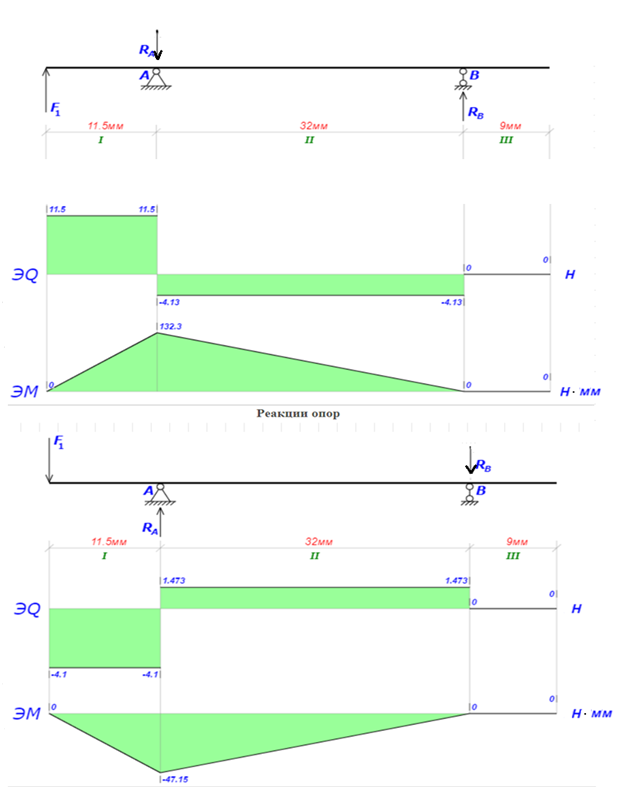
\includegraphics[max width=\textwidth]{calculations/500.png}
  \caption{Type figure caption here}
  \label{fig:500}
 \end{center}
\end{figure}
%%%
\begin{equation*}
R_{BX} \defeq \frac{\textit{F}_{\textit{t8}} \cdot S}{U} = {4.0501 \: \mathrm{N}}
\end{equation*}
%%%
\begin{equation*}
R_{AX} \defeq \textit{F}_{\textit{t8}}+R_{BX} = {15.3199 \: \mathrm{N}}
\end{equation*}
%%%
\begin{equation*}
R_{BY} \defeq \frac{\textit{F}_{\textit{r8}} \cdot S}{U} = {1.4741 \: \mathrm{N}}
\end{equation*}
%%%
\begin{equation*}
R_{AY} \defeq \textit{F}_{\textit{r8}}+R_{BY} = {5.576 \: \mathrm{N}}
\end{equation*}
%%%
\begin{equation*}
M_{ux} \defeq 130 \: \mathrm{N} \: \mathrm{mm} = {0.13 \: \mathrm{J}}
\end{equation*}
%%%
\begin{equation*}
M_{uy} \defeq 47.2 \: \mathrm{N} \: \mathrm{mm} = {0.0472 \: \mathrm{J}}
\end{equation*}
%%%
\begin{equation*}
σ_{экв} \defeq \frac{\sqrt{M_{ux}^{2}+M_{uy}^{2}+M_{V}^{2}}}{0.1 \cdot d^{3}} = {1.7638 \cdot 10^{7} \: \mathrm{Pa}}
\end{equation*}
%%%
\begin{equation*}
σ_{ud} \defeq \frac{σ_{Tshaft}}{\textit{S}_{\textit{1}}} = {5.3333 \cdot 10^{7} \: \mathrm{Pa}}
\end{equation*}
%%%
\colorbox[HTML]{FFFF80}{Условие прочности выполняется!}\newline
%%%
\colorbox[HTML]{000000}{\textbf{9.4 Расчет валов и осей на усталостную прочность:}}\newline
%%%
\colorbox[HTML]{000000}{При симметричном цикле:}\newline
%%%
\begin{equation*}
\textit{σ}_{\textit{пред1}} \defeq 0.43 \cdot σ_{Bshaft} = {2.279 \cdot 10^{8} \: \mathrm{Pa}}
\end{equation*}
%%%
\begin{equation*}
\textit{τ}_{\textit{пред1}} \defeq 0.22 \cdot σ_{Bshaft} = {1.166 \cdot 10^{8} \: \mathrm{Pa}}
\end{equation*}
%%%
\colorbox[HTML]{000000}{При отнулевом цикле:}\newline
%%%
\begin{equation*}
\textit{σ}_{\textit{пред0}} \defeq 0.6 \cdot σ_{Bshaft} = {3.18 \cdot 10^{8} \: \mathrm{Pa}}
\end{equation*}
%%%
\begin{equation*}
\textit{τ}_{\textit{пред0}} \defeq 0.32 \cdot σ_{Bshaft} = {1.696 \cdot 10^{8} \: \mathrm{Pa}}
\end{equation*}
%%%
\colorbox[HTML]{000000}{Масштабный коэффициент:}\newline
%%%
\begin{equation*}
K_{m} \defeq 0.9
\end{equation*}
%%%
\colorbox[HTML]{000000}{Коэффициенты концентрации напряжений по изгибу и кручению соответственно:}\newline
%%%
\begin{equation*}
K_{σ} \defeq 1.6
\end{equation*}
%%%
\begin{equation*}
K_{τ} \defeq 1.25
\end{equation*}
%%%
\colorbox[HTML]{000000}{Технологический коэффициент:}\newline
%%%
\begin{equation*}
K_{T} \defeq 1
\end{equation*}
%%%
\colorbox[HTML]{000000}{Коэффициент, учитывающий неточность в выборе расчетной схемы нагрузок:}\newline
%%%
\begin{equation*}
\textit{n1} \defeq 1.2
\end{equation*}
%%%
\colorbox[HTML]{000000}{Поправка на отклонения, принимаемые в расчете на прочность механических характеристик материала, , от действительных.}\newline
%%%
\begin{equation*}
\textit{n2} \defeq 1.2
\end{equation*}
%%%
\colorbox[HTML]{000000}{Степень ответственности детали и ее влияние на общею работу ПМ:}\newline
%%%
\begin{equation*}
\textit{n3} \defeq 2
\end{equation*}
%%%
\colorbox[HTML]{000000}{Запасы прочности по нормальным и касательным напряжениям:}\newline
%%%
\begin{equation*}
n_{στ} \defeq \textit{n1} \cdot \textit{n2} \cdot \textit{n3} = {2.88}
\end{equation*}
%%%
\colorbox[HTML]{000000}{Допускаемые нормальные и касательные напряжения соответственно при симметричном цикле:}\newline
%%%
\begin{equation*}
\textit{σ}_{\textit{u1}} \defeq \frac{\textit{σ}_{\textit{пред1}} \cdot K_{m}}{K_{σ} \cdot K_{T} \cdot n_{στ}} = {4.4512 \cdot 10^{7} \: \mathrm{Pa}}
\end{equation*}
%%%
\begin{equation*}
\textit{τ}_{\textit{1}} \defeq \frac{\textit{τ}_{\textit{пред1}} \cdot K_{m}}{K_{T} \cdot K_{τ} \cdot n_{στ}} = {2.915 \cdot 10^{7} \: \mathrm{Pa}}
\end{equation*}
%%%
\colorbox[HTML]{000000}{Допускаемые нормальные и касательные напряжения соответственно при отнулевом цикле:}\newline
%%%
\begin{equation*}
\textit{σ}_{\textit{u0}} \defeq \frac{\textit{σ}_{\textit{пред0}} \cdot K_{m}}{K_{σ} \cdot K_{T} \cdot n_{στ}} = {6.2109 \cdot 10^{7} \: \mathrm{Pa}}
\end{equation*}
%%%
\begin{equation*}
\textit{τ}_{\textit{0}} \defeq \frac{\textit{τ}_{\textit{пред0}} \cdot K_{m}}{K_{T} \cdot K_{τ} \cdot n_{στ}} = {4.24 \cdot 10^{7} \: \mathrm{Pa}}
\end{equation*}
%%%
\begin{figure}[h!]
 \begin{center}
  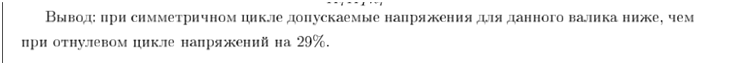
\includegraphics[max width=\textwidth]{calculations/538.png}
  \caption{Type figure caption here}
  \label{fig:538}
 \end{center}
\end{figure}
%%%
\colorbox[HTML]{000000}{Расчет радиальных подшипников на динамическую грузоподъемность:}\newline
%%%
\colorbox[HTML]{000000}{Базовая динамическая грузоподъемность:}\newline
%%%
\begin{equation*}
C \defeq 884
\end{equation*}
%%%
\colorbox[HTML]{000000}{В качестве радиальной нагрузки принимается наибольшая из результирующий реакций в опорах R,A и R,B}\newline
%%%
\begin{equation*}
R_{A} \defeq \sqrt{R_{AX}^{2}+R_{AY}^{2}} = {16.3031 \: \mathrm{N}}
\end{equation*}
%%%
\begin{equation*}
R_{B} \defeq \sqrt{R_{BX}^{2}+R_{BY}^{2}} = {4.31 \: \mathrm{N}}
\end{equation*}
%%%
\begin{equation*}
F_{r} \defeq R_{A} = {16.3031 \: \mathrm{N}}
\end{equation*}
%%%
\colorbox[HTML]{000000}{Коэффициент вращения, при вращении внутреннего кольца подшипника:}\newline
%%%
\begin{equation*}
V \defeq 1
\end{equation*}
%%%
\colorbox[HTML]{000000}{Коэффициент безопасности:}\newline
%%%
\begin{equation*}
K_{Б} \defeq 1
\end{equation*}
%%%
\colorbox[HTML]{000000}{Температурный коэффициент:}\newline
%%%
\begin{equation*}
K_{Т} \defeq 1
\end{equation*}
%%%
\colorbox[HTML]{000000}{Эквивалентная нагрузка:}\newline
%%%
\begin{equation*}
P \defeq V \cdot F_{r} \cdot K_{Б} \cdot K_{T} = {16.3031 \: \mathrm{N}}
\end{equation*}
%%%
\colorbox[HTML]{000000}{Расчетное значение динамической грузоподъемности:}\newline
%%%
\begin{equation*}
C_{р} \defeq 10^{ \operatorname{-} 2} \cdot P \cdot \left( \frac{L_{h}}{3600} \cdot 3600 \cdot n_{v} \right)^{\frac{1}{3}} = {60.9296 \: \mathrm{N}}
\end{equation*}
%%%
\colorbox[HTML]{FFFF80}{\textit{Условие на динамическую грузоподъемность выполняется!}}\newline
%%%
\colorbox[HTML]{000000}{\textbf{10. Собственный момент трения механизма.}}\newline
%%%
\colorbox[HTML]{000000}{Коэффициент трения скольжения:}\newline
%%%
\begin{equation*}
f = {0.08}
\end{equation*}
%%%
\begin{equation*}
M_{TOI} \defeq 0.040 \: \mathrm{N} \: \mathrm{m}
\end{equation*}
%%%
\begin{equation*}
M_{TOII} \defeq 0.03 \: \mathrm{N} \: \mathrm{mm} \cdot 5^{2} = {0.0008 \: \mathrm{J}}
\end{equation*}
%%%
\begin{equation*}
M_{TOIII} \defeq 0.03 \: \mathrm{N} \: \mathrm{mm} \cdot 5^{2} = {0.0008 \: \mathrm{J}}
\end{equation*}
%%%
\begin{equation*}
M_{TOIV} \defeq 0.03 \: \mathrm{N} \: \mathrm{mm} \cdot 5^{2} = {0.0008 \: \mathrm{J}}
\end{equation*}
%%%
\begin{equation*}
M_{TOV} \defeq 0.03 \: \mathrm{N} \: \mathrm{mm} \cdot 6^{2} = {0.0011 \: \mathrm{J}}
\end{equation*}
%%%
\begin{equation*}
M_{TOΣ} \defeq M_{TOI}+\frac{M_{TOII}}{\textit{i}_{\textit{12}} \cdot \textit{η}_{\textit{21}}}+\frac{M_{TOIII}}{\textit{i}_{\textit{12}} \cdot \textit{i}_{\textit{34}} \cdot \textit{η}_{\textit{21}} \cdot \textit{η}_{\textit{43}}}+\frac{M_{TOIV}}{\textit{i}_{\textit{12}} \cdot \textit{i}_{\textit{34}} \cdot \textit{i}_{\textit{56}} \cdot \textit{η}_{\textit{21}} \cdot \textit{η}_{\textit{43}} \cdot \textit{η}_{\textit{65}}}+\frac{M_{TOV}}{\textit{i}_{\textit{12}} \cdot \textit{i}_{\textit{34}} \cdot \textit{i}_{\textit{56}} \cdot \textit{i}_{\textit{78}} \cdot \textit{η}_{\textit{21}} \cdot \textit{η}_{\textit{43}} \cdot \textit{η}_{\textit{65}} \cdot \textit{η}_{\textit{78}}} = {0.0409 \: \mathrm{J}}
\end{equation*}
%%%
\colorbox[HTML]{000000}{\textbf{11. Расчет на прочность штифтового соединения:}}\newline
%%%
\colorbox[HTML]{000000}{Условие прочности штифта:}\newline
%%%
\begin{equation*}
τ_{ср} \leq τ_{dср}
\end{equation*}
%%%
\begin{equation*}
τ_{dср} \defeq 60-80 \: \mathrm{MPa}
\end{equation*}
%%%
\colorbox[HTML]{000000}{Усилие, отнесенное к одной поверхности среза штифта:}\newline
%%%
\begin{equation*}
P'_{ср} \defeq \frac{M_{V}}{d} = {59.1667 \: \mathrm{N}}
\end{equation*}
%%%
\colorbox[HTML]{000000}{Площадь поперечного сечения штифта:}\newline
%%%
\begin{equation*}
d_{шт} \defeq 1.3 \: \mathrm{mm}
\end{equation*}
%%%
\begin{equation*}
F_{шт} \defeq \frac{{\pi} \cdot d_{шт}^{2}}{4} = {1.3273 \cdot 10^{ \operatorname{-} 6} \: \mathrm{m}^{2}}
\end{equation*}
%%%
\colorbox[HTML]{000000}{Напряжение среза:}\newline
%%%
\begin{equation*}
τ_{ср} \defeq \frac{P'_{ср}}{F_{шт}} = {4.4576 \cdot 10^{7} \: \mathrm{Pa}}
\end{equation*}
%%%
\colorbox[HTML]{FFFF80}{Условие прочности штифтового соединения на срез выполняется!}\newline
%%%
\colorbox[HTML]{000000}{\textbf{12. Расчет шпонки на прочность:}}\newline
%%%
\begin{figure}[h!]
 \begin{center}
  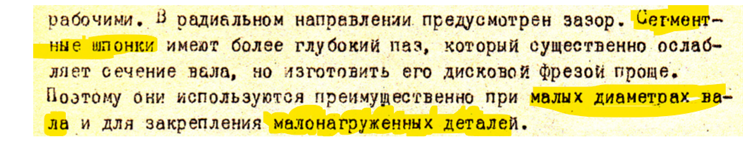
\includegraphics[max width=\textwidth]{calculations/579.png}
  \caption{Type figure caption here}
  \label{fig:579}
 \end{center}
\end{figure}
%%%
\colorbox[HTML]{000000}{Сегментная шпонка для вала диаметром 6мм}\newline
%%%
\begin{equation*}
h_{ш} \defeq 3.7 \: \mathrm{mm}
\end{equation*}
%%%
\begin{equation*}
b_{ш} \defeq 2 \: \mathrm{mm}
\end{equation*}
%%%
\begin{equation*}
D \defeq 10 \: \mathrm{mm}
\end{equation*}
%%%
\begin{equation*}
\textit{t}_{\textit{1}} \defeq 2.9 \: \mathrm{mm}
\end{equation*}
%%%
\begin{equation*}
\textit{t}_{\textit{2}} \defeq 1.0 \: \mathrm{mm}
\end{equation*}
%%%
\begin{figure}[h!]
 \begin{center}
  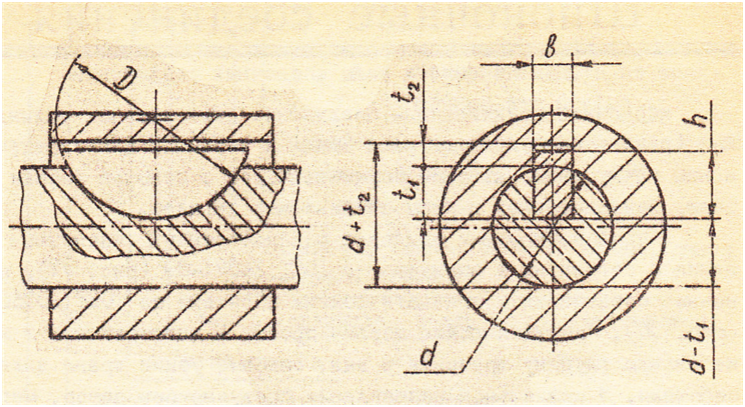
\includegraphics[max width=\textwidth]{calculations/586.png}
  \caption{Type figure caption here}
  \label{fig:586}
 \end{center}
\end{figure}
%%%
\begin{equation*}
σ_{dсм} \defeq 150-180 \: \mathrm{MPa}
\end{equation*}
%%%
\begin{equation*}
σ_{см} \defeq 2 \cdot \frac{M_{V}}{d \cdot \left( h_{ш}-\textit{t}_{\textit{1}} \right) \cdot D} = {1.4792 \cdot 10^{7} \: \mathrm{Pa}}
\end{equation*}
%%%
\colorbox[HTML]{FFFF80}{Условие прочности шпонки на смятие удовлетворяется!}\newline
%%%
\colorbox[HTML]{000000}{Сегментная шпонка для вала диаметром 4мм}\newline
%%%
\begin{equation*}
h_{ш} \defeq 2.6 \: \mathrm{mm}
\end{equation*}
%%%
\begin{equation*}
b_{ш} \defeq 1.5 \: \mathrm{mm}
\end{equation*}
%%%
\begin{equation*}
D \defeq 4 \: \mathrm{mm}
\end{equation*}
%%%
\begin{equation*}
\textit{t}_{\textit{1}} \defeq 1.0 \: \mathrm{mm}
\end{equation*}
%%%
\begin{equation*}
\textit{t}_{\textit{2}} \defeq 0.6 \: \mathrm{mm}
\end{equation*}
%%%
\colorbox[HTML]{000000}{\textbf{13. Расчет на прочность винтового соединения:}}\newline
%%%
\colorbox[HTML]{000000}{Условия прочности:}\newline
%%%
\colorbox[HTML]{000000}{Для разрыва стержня:}\newline
%%%
\begin{equation*}
σ_{пр} \leq σ_{др}
\end{equation*}
%%%
\colorbox[HTML]{000000}{Для среза витков:}\newline
%%%
\begin{equation*}
τ_{ср} \leq τ_{дср}
\end{equation*}
%%%
\colorbox[HTML]{000000}{Для смятия поверхности витков:}\newline
%%%
\begin{equation*}
σ_{см} \leq σ_{дсм}
\end{equation*}
%%%
\colorbox[HTML]{000000}{Q - усилие затяжки резьбового соединения}\newline
%%%
\begin{equation*}
Q \defeq 258 \: \mathrm{N}
\end{equation*}
%%%
\colorbox[HTML]{000000}{F - площадь поперечного сечения винта}\newline
%%%
\begin{equation*}
d_{в} \defeq 2.5 \: \mathrm{mm}
\end{equation*}
%%%
\begin{equation*}
F \defeq 0.5 \cdot d_{в}^{2} = {3.125 \cdot 10^{ \operatorname{-} 6} \: \mathrm{m}^{2}}
\end{equation*}
%%%
\colorbox[HTML]{000000}{Определение приведенного напряжения в стержне винта:}\newline
%%%
\begin{equation*}
σ_{пр} \defeq 1.3 \cdot \frac{Q}{F} = {1.0733 \cdot 10^{8} \: \mathrm{Pa}}
\end{equation*}
%%%
\begin{equation*}
\textit{d}_{\textit{1в}} \defeq d_{в} = {0.0025 \: \mathrm{m}}
\end{equation*}
%%%
\begin{equation*}
d_{г} \defeq \textit{d}_{\textit{1в}} = {0.0025 \: \mathrm{m}}
\end{equation*}
%%%
\colorbox[HTML]{000000}{Длина свинчивания:}\newline
%%%
\begin{equation*}
L_{св} \defeq \textit{d}_{\textit{1в}} = {0.0025 \: \mathrm{m}}
\end{equation*}
%%%
\colorbox[HTML]{000000}{Определение напряжения среза:}\newline
%%%
\colorbox[HTML]{000000}{Срез витков винта происходит по цилиндру диаметра d, а гайки по внутреннему диаметру d1}\newline
%%%
\colorbox[HTML]{000000}{Для винта:}\newline
%%%
\begin{equation*}
τ_{срв} \defeq \frac{Q}{{\pi} \cdot \textit{d}_{\textit{1в}} \cdot 0.75 \cdot L_{св}} = {1.752 \cdot 10^{7} \: \mathrm{Pa}}
\end{equation*}
%%%
\colorbox[HTML]{000000}{Для гайки:}\newline
%%%
\begin{equation*}
τ_{срг} \defeq \frac{Q}{{\pi} \cdot d_{г} \cdot 0.88 \cdot L_{св}} = {1.4932 \cdot 10^{7} \: \mathrm{Pa}}
\end{equation*}
%%%
\begin{equation*}
d \defeq \textit{d}_{\textit{1в}} = {0.0025 \: \mathrm{m}}
\end{equation*}
%%%
\colorbox[HTML]{000000}{Диаметр винта без высоты резьбы:}\newline
%%%
\begin{equation*}
\textit{d}_{\textit{1}} \defeq 2.1 \: \mathrm{mm} = {0.0021 \: \mathrm{m}}
\end{equation*}
%%%
\colorbox[HTML]{000000}{(ГОСТ 24705-2004)}\newline
%%%
\colorbox[HTML]{000000}{0,75 и 0,88 - коэффициенты полноты резьбы, учитывающие отношение толщины витка на цилиндре, по которому происходит срез витков, к шагу резьбы}\newline
%%%
\colorbox[HTML]{000000}{Определение напряжения смятия:}\newline
%%%
\colorbox[HTML]{000000}{Шаг резьбы:}\newline
%%%
\begin{equation*}
p \defeq 0.45 \: \mathrm{mm}
\end{equation*}
%%%
\begin{equation*}
z \defeq \frac{L_{св}}{p} = {5.5556}
\end{equation*}
%%%
\begin{equation*}
σ_{см} \defeq 4 \cdot \frac{Q}{{\pi} \cdot \left( d^{2}-\textit{d}_{\textit{1}}^{2} \right) \cdot z \cdot 1000} = {32135.4589 \: \mathrm{Pa}}
\end{equation*}
%%%
\colorbox[HTML]{000000}{В расчетах на смятие и на срез витков условно предполагают, что общая нагрузка Q распределяется поровну между всеми рабочими витками. Неточность такого предположения компенсируется уменьшением допускаемых напряжений.}\newline
%%%
\colorbox[HTML]{000000}{Определение допускаемых напряжений:}\newline
%%%
\colorbox[HTML]{000000}{Предел текучести винтов:}\newline
%%%
\begin{equation*}
σ_{твинтов} \defeq 240 \: \mathrm{MPa}
\end{equation*}
%%%
\colorbox[HTML]{000000}{Коэффициент запаса:}\newline
%%%
\begin{equation*}
n \defeq 1.5
\end{equation*}
%%%
\begin{equation*}
σ_{др} \defeq \frac{σ_{твинтов}}{n} = {1.6 \cdot 10^{8} \: \mathrm{Pa}}
\end{equation*}
%%%
\begin{equation*}
τ_{дср} \defeq 0.75 \cdot σ_{др} = {1.2 \cdot 10^{8} \: \mathrm{Pa}}
\end{equation*}
%%%
\begin{equation*}
σ_{дсм} \defeq 0.4 \cdot σ_{др} = {6.4 \cdot 10^{7} \: \mathrm{Pa}}
\end{equation*}
%%%
\colorbox[HTML]{000000}{\textbf{14. Расчет фрикционной муфты:}}\newline
%%%
\colorbox[HTML]{000000}{Режим работы 1 - постоянная нагрузка}\newline
%%%
\begin{equation*}
r_{HAP} \defeq 25 \: \mathrm{mm}
\end{equation*}
%%%
\begin{equation*}
r_{BH} \defeq 18 \: \mathrm{mm}
\end{equation*}
%%%
\colorbox[HTML]{000000}{Крутящий момент, при котором начинается проскальзывание одной полумуфты относительно другой:}\newline
%%%
\begin{equation*}
M_{муфты} \defeq M_{Σ} = {0.355 \: \mathrm{J}}
\end{equation*}
%%%
\colorbox[HTML]{000000}{Число поверхностей трения:}\newline
%%%
\begin{equation*}
n_{пт} \defeq 2
\end{equation*}
%%%
\colorbox[HTML]{000000}{Коэффициент трения скольжения пары материалов:}\newline
%%%
\begin{equation*}
f_{муфты} \defeq 0.1
\end{equation*}
%%%
\colorbox[HTML]{000000}{сталь по стали}\newline
%%%
\begin{equation*}
k_{ЗАП} \defeq 1.0
\end{equation*}
%%%
\colorbox[HTML]{000000}{Средний радиус площадки контакта:}\newline
%%%
\begin{equation*}
r_{ср} \defeq \frac{r_{HAP}+r_{BH}}{2} = {0.0215 \: \mathrm{m}}
\end{equation*}
%%%
\colorbox[HTML]{000000}{Сила пружины при рабочей деформации:}\newline
%%%
\begin{equation*}
\textit{F}_{\textit{2пружины}} \defeq \frac{k_{ЗАП} \cdot M_{муфты}}{n_{пт} \cdot f_{муфты} \cdot r_{ср}} = {82.5581 \: \mathrm{N}}
\end{equation*}
%%%
\colorbox[HTML]{000000}{площадь кольца, по которому контактируют детали муфты}\newline
%%%
\begin{equation*}
F_{Kмуфты} \defeq {\pi} \cdot \left( r_{HAP}^{2}-r_{BH}^{2} \right) = {0.0009 \: \mathrm{m}^{2}}
\end{equation*}
%%%
\colorbox[HTML]{000000}{Допускаемое давление:}\newline
%%%
\begin{equation*}
p_{д} \defeq 1.5 \: \mathrm{MPa}
\end{equation*}
%%%
\colorbox[HTML]{000000}{Удельное давление, возникающее на поверхностях трения:}\newline
%%%
\begin{equation*}
p_{муфты} \defeq \frac{\textit{F}_{\textit{2пружины}}}{F_{Kмуфты}} = {87305.887 \: \mathrm{Pa}}
\end{equation*}
%%%
\colorbox[HTML]{000000}{\textbf{Расчет пружины:}}\newline
%%%
\colorbox[HTML]{000000}{1. Сила пружины при максимальной деформации:}\newline
%%%
\begin{equation*}
\textit{F}_{\textit{3пружины}} \defeq 1.2 \cdot \textit{F}_{\textit{2пружины}} = {99.0698 \: \mathrm{N}}
\end{equation*}
%%%
\colorbox[HTML]{000000}{Средний диаметр пружины ( подбирается по эскизу ):}\newline
%%%
\begin{equation*}
D_{пружины} \defeq 12.0 \: \mathrm{mm} = {0.012 \: \mathrm{m}}
\end{equation*}
%%%
\colorbox[HTML]{000000}{2. Выбираем предварительное значение индекса пружины iпр: }\newline
%%%
\begin{equation*}
i_{пр} \defeq 6
\end{equation*}
%%%
\colorbox[HTML]{000000}{(ГОСТ 13765-86)}\newline
%%%
\colorbox[HTML]{000000}{3. предварительное значение диаметра проволоки:}\newline
%%%
\begin{equation*}
d_{пр} \defeq \frac{D_{пружины}}{i_{пр}} = {0.002 \: \mathrm{m}}
\end{equation*}
%%%
\colorbox[HTML]{000000}{4. Выбираем ближайшее значение диаметра проволоки d по таблице ГОСТ 9389-75}\newline
%%%
\begin{equation*}
d_{проволоки} \defeq 2.0 \: \mathrm{mm} = {0.002 \: \mathrm{m}}
\end{equation*}
%%%
\begin{figure}[h!]
 \begin{center}
  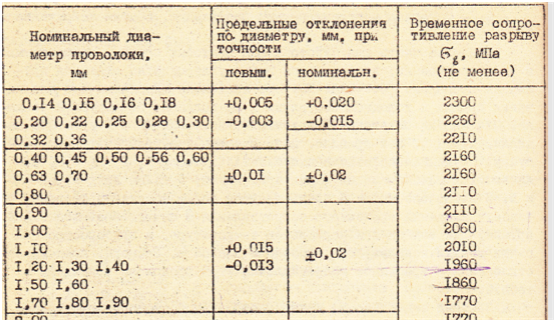
\includegraphics[max width=\textwidth]{calculations/674.png}
  \caption{Type figure caption here}
  \label{fig:674}
 \end{center}
\end{figure}
%%%
\colorbox[HTML]{000000}{5. Действительное значение индекса пружины:}\newline
%%%
\begin{equation*}
i_{пружины} \defeq \frac{D_{пружины}}{d_{проволоки}} = {6}
\end{equation*}
%%%
\colorbox[HTML]{000000}{6. Коэффициент, учитывающий кривизну витка пружины k}\newline
%%%
\begin{equation*}
k \defeq \frac{4 \cdot i_{пружины}-1}{4 \cdot i_{пружины}-4}+\frac{0.615}{i_{пружины}} = {1.2525}
\end{equation*}
%%%
\colorbox[HTML]{000000}{7. Допускаемое касательное напряжение для выбранного диаметра проволоки:}\newline
%%%
\colorbox[HTML]{000000}{предел прочности:}\newline
%%%
\begin{equation*}
σ_{Впружины} \defeq 1770 \: \mathrm{MPa} = {1.77 \cdot 10^{9} \: \mathrm{Pa}}
\end{equation*}
%%%
\begin{equation*}
τ_{д} \defeq 0.32 \cdot σ_{Впружины} = {5.664 \cdot 10^{8} \: \mathrm{Pa}}
\end{equation*}
%%%
\colorbox[HTML]{000000}{8. Минимально возможный по условию прочности диаметр проволоки:}\newline
%%%
\begin{equation*}
d_{min} \defeq 1.6 \cdot \sqrt{\frac{\textit{F}_{\textit{3пружины}} \cdot i_{пружины} \cdot k}{τ_{д}}} = {0.0018 \: \mathrm{m}}
\end{equation*}
%%%
\colorbox[HTML]{000000}{9. Проверяем выбранное значение диаметра проволоки по условию прочности }\newline
%%%
\begin{equation*}
d_{проволоки} \geq d_{min}
\end{equation*}
%%%
\colorbox[HTML]{000000}{Если условие не выполняется, уменьшаем значение iпр и повторяем расчет с пункта 2}\newline
%%%
\colorbox[HTML]{000000}{10. Определяем число рабочих витков n}\newline
%%%
\colorbox[HTML]{000000}{S2 – рабочая деформация пружины, назначается в пределах 4…6 мм}\newline
%%%
\begin{equation*}
\textit{S}_{\textit{2пружины}} \defeq 5 \: \mathrm{mm}
\end{equation*}
%%%
\begin{equation*}
n_{витков} \defeq \frac{10125 \cdot \textit{S}_{\textit{2пружины}} \cdot d_{проволоки}}{\textit{F}_{\textit{2пружины}} \cdot i_{пружины}^{3}} = {5.6778 \cdot 10^{ \operatorname{-} 6} \: \frac{\mathrm{m} \: \mathrm{s}^{2}}{\mathrm{kg}}}
\end{equation*}
%%%
\begin{figure}[h!]
 \begin{center}
  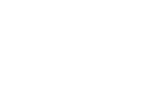
\includegraphics[max width=\textwidth]{calculations/692.png}
  \caption{Type figure caption here}
  \label{fig:692}
 \end{center}
\end{figure}
%%%
\colorbox[HTML]{000000}{11. Округлить число витков до ближайшего необходимого значения.}\newline
%%%
\begin{equation*}
n_{витков} \defeq 5
\end{equation*}
%%%
\colorbox[HTML]{000000}{12. Для принятого числа витков рассчитываем уточнённое значение рабочей деформации }\newline
%%%
\colorbox[HTML]{000000}{модуль сдвига, для стальной пружинной проволоки }\newline
%%%
\begin{equation*}
G_{проволоки} \defeq 81000 \: \mathrm{MPa}
\end{equation*}
%%%
\begin{equation*}
\textit{S}_{\textit{2пружины}} \defeq \frac{8 \cdot \textit{F}_{\textit{2пружины}} \cdot n_{витков} \cdot D_{пружины}^{3}}{G_{проволоки} \cdot d_{проволоки}^{4}} = {0.0044 \: \mathrm{m}}
\end{equation*}
%%%
\colorbox[HTML]{000000}{13. Длина пружины при полностью поджатых витках }\newline
%%%
\begin{equation*}
L \defeq d_{проволоки} \cdot \left( n_{витков}+1 \right) = {0.012 \: \mathrm{m}}
\end{equation*}
%%%
\colorbox[HTML]{000000}{14. Жёсткость пружины}\newline
%%%
\begin{equation*}
C_{пружины} \defeq \frac{\textit{F}_{\textit{2пружины}}}{\textit{S}_{\textit{2пружины}}} = {18750 \: \mathrm{m} \: \mathrm{Pa}}
\end{equation*}
%%%
\colorbox[HTML]{000000}{\textbf{15. Расчет приведенного момента инерции.}}\newline
%%%
\colorbox[HTML]{000000}{Приведенный момент инерции ротора двигателя:}\newline
%%%
\begin{equation*}
J_{пррот} \defeq J = {8.69 \cdot 10^{ \operatorname{-} 7} \: \mathrm{kg} \: \mathrm{m}^{2}}
\end{equation*}
%%%
\begin{equation*}
{\rho} \defeq 7.85 \cdot 10^{ \operatorname{-} 6} \: \frac{\mathrm{kg}}{\mathrm{mm}^{3}}
\end{equation*}
%%%
\colorbox[HTML]{000000}{Диаметры ступиц зубчатых колес:}\newline
%%%
\colorbox[HTML]{000000}{Ширина венцов зубчатых колес:}\newline
%%%
\begin{equation*}
\textit{d}_{\textit{ст1}} \defeq 8 \: \mathrm{mm} = {0.008 \: \mathrm{m}}
\end{equation*}
%%%
\begin{equation*}
\textit{b}_{\textit{1}} \defeq 2 \: \mathrm{mm}
\end{equation*}
%%%
\begin{equation*}
\textit{d}_{\textit{ст2}} \defeq 9 \: \mathrm{mm} = {0.009 \: \mathrm{m}}
\end{equation*}
%%%
\begin{equation*}
\textit{b}_{\textit{2}} \defeq \textit{b}_{\textit{1}} = {0.002 \: \mathrm{m}}
\end{equation*}
%%%
\begin{equation*}
\textit{d}_{\textit{ст3}} \defeq 9 \: \mathrm{mm} = {0.009 \: \mathrm{m}}
\end{equation*}
%%%
\begin{equation*}
\textit{b}_{\textit{3}} \defeq \textit{b}_{\textit{1}} = {0.002 \: \mathrm{m}}
\end{equation*}
%%%
\begin{equation*}
\textit{d}_{\textit{ст4}} \defeq 9 \: \mathrm{mm} = {0.009 \: \mathrm{m}}
\end{equation*}
%%%
\begin{equation*}
\textit{b}_{\textit{4}} \defeq \textit{b}_{\textit{1}} = {0.002 \: \mathrm{m}}
\end{equation*}
%%%
\begin{equation*}
\textit{d}_{\textit{ст5}} \defeq 9 \: \mathrm{mm} = {0.009 \: \mathrm{m}}
\end{equation*}
%%%
\begin{equation*}
\textit{b}_{\textit{5}} \defeq \textit{b}_{\textit{1}} = {0.002 \: \mathrm{m}}
\end{equation*}
%%%
\begin{equation*}
\textit{d}_{\textit{ст6}} \defeq 9 \: \mathrm{mm} = {0.009 \: \mathrm{m}}
\end{equation*}
%%%
\begin{equation*}
\textit{b}_{\textit{6}} \defeq \textit{b}_{\textit{1}} = {0.002 \: \mathrm{m}}
\end{equation*}
%%%
\begin{equation*}
\textit{d}_{\textit{ст7}} \defeq 9 \: \mathrm{mm} = {0.009 \: \mathrm{m}}
\end{equation*}
%%%
\begin{equation*}
\textit{b}_{\textit{7}} \defeq \textit{b}_{\textit{1}} = {0.002 \: \mathrm{m}}
\end{equation*}
%%%
\begin{equation*}
\textit{d}_{\textit{ст8}} \defeq 10 \: \mathrm{mm}
\end{equation*}
%%%
\begin{equation*}
\textit{b}_{\textit{8}} \defeq 0.003 \: \mathrm{m}
\end{equation*}
%%%
\begin{equation*}
d_{стpov} \defeq 10 \: \mathrm{mm}
\end{equation*}
%%%
\begin{equation*}
b_{pov} \defeq 0.002 \: \mathrm{m}
\end{equation*}
%%%
\colorbox[HTML]{000000}{Диаметры отвертстий:}\newline
%%%
\colorbox[HTML]{000000}{Длины ступиц:}\newline
%%%
\begin{equation*}
\textit{d}_{\textit{отв1}} \defeq 4 \: \mathrm{mm}
\end{equation*}
%%%
\begin{equation*}
\textit{l}_{\textit{ст1}} \defeq 5 \: \mathrm{mm}
\end{equation*}
%%%
\begin{equation*}
\textit{l}_{\textit{ст5}} \defeq 6 \: \mathrm{mm}
\end{equation*}
%%%
\begin{equation*}
\textit{d}_{\textit{отв2}} \defeq 5 \: \mathrm{mm}
\end{equation*}
%%%
\begin{equation*}
\textit{l}_{\textit{ст2}} \defeq 6 \: \mathrm{mm}
\end{equation*}
%%%
\begin{equation*}
\textit{l}_{\textit{ст6}} \defeq 6.5 \: \mathrm{mm}
\end{equation*}
%%%
\begin{equation*}
\textit{d}_{\textit{отв3}} \defeq \textit{d}_{\textit{отв2}} = {0.005 \: \mathrm{m}}
\end{equation*}
%%%
\begin{equation*}
\textit{d}_{\textit{отв4}} \defeq \textit{d}_{\textit{отв3}} = {0.005 \: \mathrm{m}}
\end{equation*}
%%%
\begin{equation*}
\textit{l}_{\textit{ст3}} \defeq 6.5 \: \mathrm{mm}
\end{equation*}
%%%
\begin{equation*}
\textit{l}_{\textit{ст7}} \defeq 6.5 \: \mathrm{mm}
\end{equation*}
%%%
\begin{equation*}
\textit{d}_{\textit{отв5}} \defeq \textit{d}_{\textit{отв4}} = {0.005 \: \mathrm{m}}
\end{equation*}
%%%
\begin{equation*}
\textit{l}_{\textit{ст4}} \defeq 6.5 \: \mathrm{mm}
\end{equation*}
%%%
\begin{equation*}
\textit{l}_{\textit{ст8}} \defeq 0 \: \mathrm{mm}
\end{equation*}
%%%
\begin{equation*}
\textit{d}_{\textit{отв6}} \defeq \textit{d}_{\textit{отв5}} = {0.005 \: \mathrm{m}}
\end{equation*}
%%%
\begin{equation*}
l_{стpov} \defeq 6 \: \mathrm{mm}
\end{equation*}
%%%
\begin{equation*}
\textit{d}_{\textit{отв7}} \defeq \textit{d}_{\textit{отв6}} = {0.005 \: \mathrm{m}}
\end{equation*}
%%%
\begin{equation*}
\textit{d}_{\textit{отв8}} \defeq 6 \: \mathrm{mm} = {0.006 \: \mathrm{m}}
\end{equation*}
%%%
\begin{equation*}
d_{отвpov} \defeq 6 \: \mathrm{mm}
\end{equation*}
%%%
\colorbox[HTML]{000000}{Массы зубчатых колес:}\newline
%%%
\begin{equation*}
\textit{m}_{\textit{1}} \defeq {\rho} \cdot {\pi} \cdot \left( \textit{b}_{\textit{1}} \cdot \frac{\left( \textit{d}_{\textit{ст1}}^{2}-\textit{d}_{\textit{отв1}}^{2} \right)}{4}+\textit{l}_{\textit{ст1}} \cdot \left( \frac{\textit{d}_{\textit{ст1}}^{2}-\textit{d}_{\textit{отв1}}^{2}}{4} \right) \right) = {0.0021 \: \mathrm{kg}}
\end{equation*}
%%%
\begin{equation*}
\textit{m}_{\textit{2}} \defeq {\rho} \cdot {\pi} \cdot \left( \textit{b}_{\textit{2}} \cdot \frac{\left( \textit{d}_{\textit{ст2}}^{2}-\textit{d}_{\textit{отв2}}^{2} \right)}{4}+\textit{l}_{\textit{ст2}} \cdot \left( \frac{\textit{d}_{\textit{ст2}}^{2}-\textit{d}_{\textit{отв2}}^{2}}{4} \right) \right) = {0.0028 \: \mathrm{kg}}
\end{equation*}
%%%
\begin{equation*}
\textit{m}_{\textit{3}} \defeq {\rho} \cdot {\pi} \cdot \left( \textit{b}_{\textit{3}} \cdot \frac{\left( \textit{d}_{\textit{ст3}}^{2}-\textit{d}_{\textit{отв3}}^{2} \right)}{4}+\textit{l}_{\textit{ст3}} \cdot \left( \frac{\textit{d}_{\textit{ст3}}^{2}-\textit{d}_{\textit{отв3}}^{2}}{4} \right) \right) = {0.0029 \: \mathrm{kg}}
\end{equation*}
%%%
\begin{equation*}
\textit{m}_{\textit{4}} \defeq {\rho} \cdot {\pi} \cdot \left( \textit{b}_{\textit{4}} \cdot \frac{\left( \textit{d}_{\textit{ст4}}^{2}-\textit{d}_{\textit{отв4}}^{2} \right)}{4}+\textit{l}_{\textit{ст4}} \cdot \left( \frac{\textit{d}_{\textit{ст4}}^{2}-\textit{d}_{\textit{отв4}}^{2}}{4} \right) \right) = {0.0029 \: \mathrm{kg}}
\end{equation*}
%%%
\begin{equation*}
\textit{m}_{\textit{5}} \defeq {\rho} \cdot {\pi} \cdot \left( \textit{b}_{\textit{5}} \cdot \frac{\left( \textit{d}_{\textit{ст5}}^{2}-\textit{d}_{\textit{отв5}}^{2} \right)}{4}+\textit{l}_{\textit{ст5}} \cdot \left( \frac{\textit{d}_{\textit{ст5}}^{2}-\textit{d}_{\textit{отв5}}^{2}}{4} \right) \right) = {0.0028 \: \mathrm{kg}}
\end{equation*}
%%%
\begin{equation*}
\textit{m}_{\textit{6}} \defeq {\rho} \cdot {\pi} \cdot \left( \textit{b}_{\textit{6}} \cdot \frac{\left( \textit{d}_{\textit{ст6}}^{2}-\textit{d}_{\textit{отв6}}^{2} \right)}{4}+\textit{l}_{\textit{ст6}} \cdot \left( \frac{\textit{d}_{\textit{ст6}}^{2}-\textit{d}_{\textit{отв6}}^{2}}{4} \right) \right) = {0.0029 \: \mathrm{kg}}
\end{equation*}
%%%
\begin{equation*}
\textit{m}_{\textit{7}} \defeq {\rho} \cdot {\pi} \cdot \left( \textit{b}_{\textit{7}} \cdot \frac{\left( \textit{d}_{\textit{ст7}}^{2}-\textit{d}_{\textit{отв7}}^{2} \right)}{4}+\textit{l}_{\textit{ст7}} \cdot \left( \frac{\textit{d}_{\textit{ст7}}^{2}-\textit{d}_{\textit{отв7}}^{2}}{4} \right) \right) = {0.0029 \: \mathrm{kg}}
\end{equation*}
%%%
\begin{equation*}
\textit{m}_{\textit{8}} \defeq {\rho} \cdot {\pi} \cdot \left( \textit{b}_{\textit{8}} \cdot \frac{\left( \textit{d}_{\textit{ст8}}^{2}-\textit{d}_{\textit{отв8}}^{2} \right)}{4}+\textit{l}_{\textit{ст8}} \cdot \left( \frac{\textit{d}_{\textit{ст8}}^{2}-\textit{d}_{\textit{отв8}}^{2}}{4} \right) \right) = {0.0012 \: \mathrm{kg}}
\end{equation*}
%%%
\begin{equation*}
m_{pov} \defeq {\rho} \cdot {\pi} \cdot \left( \textit{b}_{\textit{1}} \cdot \frac{\left( d_{стpov}^{2}-d_{отвpov}^{2} \right)}{4}+l_{стpov} \cdot \left( \frac{d_{стpov}^{2}-d_{отвpov}^{2}}{4} \right) \right) = {0.0032 \: \mathrm{kg}}
\end{equation*}
%%%
\colorbox[HTML]{000000}{Моменты инерции зубчатых колес:}\newline
%%%
\begin{equation*}
\textit{J}_{\textit{1}} \defeq \frac{\textit{m}_{\textit{1}} \cdot \left( \frac{\textit{d}_{\textit{a1}}}{2} \right)^{2}}{2} = {8.5209 \cdot 10^{ \operatorname{-} 8} \: \mathrm{kg} \: \mathrm{m}^{2}}
\end{equation*}
%%%
\begin{equation*}
\textit{J}_{\textit{2}} \defeq \frac{\textit{m}_{\textit{2}} \cdot \left( \frac{\textit{d}_{\textit{a2}}}{2} \right)^{2}}{2} = {2.6798 \cdot 10^{ \operatorname{-} 7} \: \mathrm{kg} \: \mathrm{m}^{2}}
\end{equation*}
%%%
\begin{equation*}
\textit{J}_{\textit{3}} \defeq \frac{\textit{m}_{\textit{3}} \cdot \left( \frac{\textit{d}_{\textit{a3}}}{2} \right)^{2}}{2} = {1.2071 \cdot 10^{ \operatorname{-} 7} \: \mathrm{kg} \: \mathrm{m}^{2}}
\end{equation*}
%%%
\begin{equation*}
\textit{J}_{\textit{4}} \defeq \frac{\textit{m}_{\textit{4}} \cdot \left( \frac{\textit{d}_{\textit{a4}}}{2} \right)^{2}}{2} = {3.7236 \cdot 10^{ \operatorname{-} 7} \: \mathrm{kg} \: \mathrm{m}^{2}}
\end{equation*}
%%%
\begin{equation*}
\textit{J}_{\textit{5}} \defeq \frac{\textit{m}_{\textit{5}} \cdot \left( \frac{\textit{d}_{\textit{a5}}}{2} \right)^{2}}{2} = {1.1361 \cdot 10^{ \operatorname{-} 7} \: \mathrm{kg} \: \mathrm{m}^{2}}
\end{equation*}
%%%
\begin{equation*}
\textit{J}_{\textit{6}} \defeq \frac{\textit{m}_{\textit{6}} \cdot \left( \frac{\textit{d}_{\textit{a6}}}{2} \right)^{2}}{2} = {7.7152 \cdot 10^{ \operatorname{-} 7} \: \mathrm{kg} \: \mathrm{m}^{2}}
\end{equation*}
%%%
\begin{equation*}
\textit{J}_{\textit{7}} \defeq \frac{\textit{m}_{\textit{7}} \cdot \left( \frac{\textit{d}_{\textit{a7}}}{2} \right)^{2}}{2} = {1.2071 \cdot 10^{ \operatorname{-} 7} \: \mathrm{kg} \: \mathrm{m}^{2}}
\end{equation*}
%%%
\begin{equation*}
\textit{J}_{\textit{8}} \defeq \frac{\textit{m}_{\textit{8}} \cdot \left( \frac{\textit{d}_{\textit{a8}}}{2} \right)^{2}}{2} = {6.2248 \cdot 10^{ \operatorname{-} 7} \: \mathrm{kg} \: \mathrm{m}^{2}}
\end{equation*}
%%%
\begin{equation*}
d_{pov} \defeq 30 \: \mathrm{mm}
\end{equation*}
%%%
\begin{equation*}
J_{pov} \defeq \frac{m_{pov} \cdot \left( \frac{d_{pov}}{2} \right)^{2}}{2} = {3.5513 \cdot 10^{ \operatorname{-} 7} \: \mathrm{kg} \: \mathrm{m}^{2}}
\end{equation*}
%%%
\colorbox[HTML]{000000}{Приведенный к первому колесу момент инерции редуктора}\newline
%%%
\begin{equation*}
J_{прред} \defeq \textit{J}_{\textit{1}}+\frac{\textit{J}_{\textit{2}}+\textit{J}_{\textit{3}}}{\textit{i}_{\textit{12}}^{2}}+\frac{\textit{J}_{\textit{4}}+\textit{J}_{\textit{5}}}{\left( \textit{i}_{\textit{12}} \cdot \textit{i}_{\textit{34}} \right)^{2}}+\frac{\textit{J}_{\textit{6}}+\textit{J}_{\textit{7}}}{\left( \textit{i}_{\textit{12}} \cdot \textit{i}_{\textit{34}} \cdot \textit{i}_{\textit{56}} \right)^{2}}+\frac{\textit{J}_{\textit{8}}+J_{pov}}{\left( \textit{i}_{\textit{12}} \cdot \textit{i}_{\textit{34}} \cdot \textit{i}_{\textit{56}} \cdot \textit{i}_{\textit{78}} \right)^{2}} = {2.9836 \cdot 10^{ \operatorname{-} 7} \: \mathrm{kg} \: \mathrm{m}^{2}}
\end{equation*}
%%%
\colorbox[HTML]{000000}{Приведенный момент инерции механизма рассчитывается по формуле:}\newline
%%%
\begin{equation*}
J_{пр} \defeq J_{пррот}+J_{прред} = {1.1674 \cdot 10^{ \operatorname{-} 6} \: \mathrm{kg} \: \mathrm{m}^{2}}
\end{equation*}
%%%
\colorbox[HTML]{000000}{\textbf{16. Расчет времени разгона механизма:}}\newline
%%%
\colorbox[HTML]{000000}{Скорость вращения вала двигателя:}\newline
%%%
\begin{equation*}
ω_{дв} \defeq 2 \cdot {\pi} \cdot n_{DV} = {471.2389 \: \mathrm{Hz}}
\end{equation*}
%%%
\colorbox[HTML]{000000}{Жесткость механической характеристики электродвигателя:}\newline
%%%
\begin{equation*}
K \defeq \frac{M_{P}-M_{DV}}{ω_{дв}} = {0.0004 \: \mathrm{s} \: \mathrm{J}}
\end{equation*}
%%%
\colorbox[HTML]{000000}{Костанта времени разгона:}\newline
%%%
\begin{equation*}
T \defeq \frac{J_{пр}}{K} = {0.0027 \: \mathrm{s}}
\end{equation*}
%%%
\colorbox[HTML]{000000}{Время разгона:}\newline
%%%
\begin{equation*}
t \defeq 3 \cdot T = {0.008 \: \mathrm{s}}
\end{equation*}
%%%
\colorbox[HTML]{000000}{17. Кинематическая погрешность передачи.}\newline
%%%
\begin{figure}[h!]
 \begin{center}
  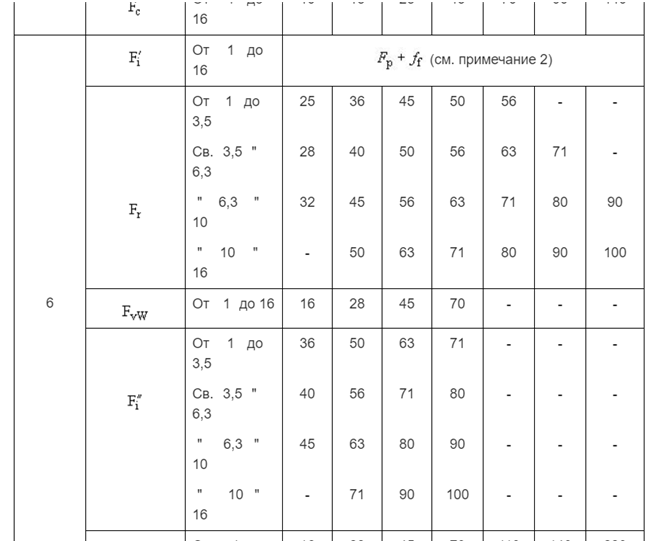
\includegraphics[max width=\textwidth]{calculations/782.png}
  \caption{Type figure caption here}
  \label{fig:782}
 \end{center}
\end{figure}
%%%
\begin{figure}[h!]
 \begin{center}
  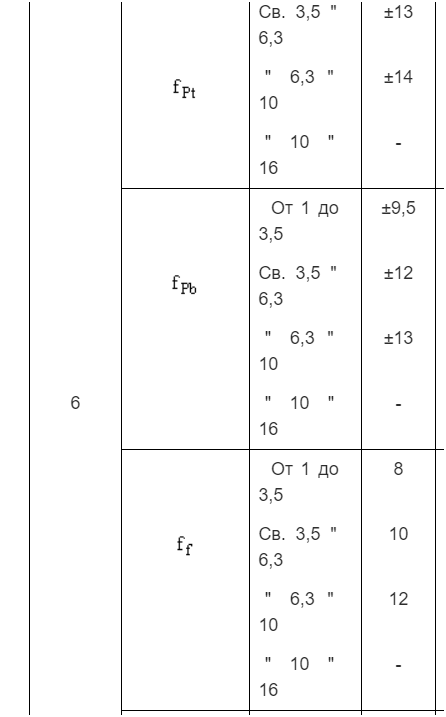
\includegraphics[max width=\textwidth]{calculations/783.png}
  \caption{Type figure caption here}
  \label{fig:783}
 \end{center}
\end{figure}
%%%
\begin{equation*}
f_{f} \defeq 8
\end{equation*}
%%%
\begin{figure}[h!]
 \begin{center}
  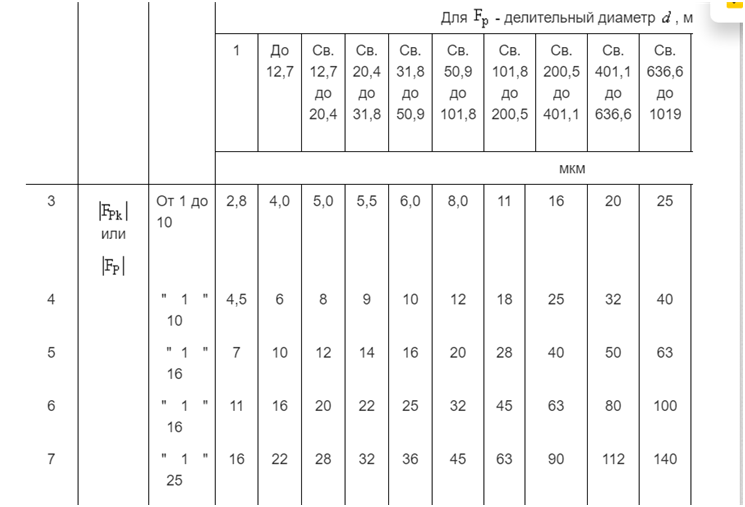
\includegraphics[max width=\textwidth]{calculations/785.png}
  \caption{Type figure caption here}
  \label{fig:785}
 \end{center}
\end{figure}
%%%
\begin{equation*}
\textit{F}_{\textit{p1}} \defeq 20
\end{equation*}
%%%
\begin{equation*}
\textit{F}_{\textit{p5}} \defeq \textit{F}_{\textit{p1}} = {20}
\end{equation*}
%%%
\begin{equation*}
\textit{F}_{\textit{p2}} \defeq 22
\end{equation*}
%%%
\begin{equation*}
\textit{F}_{\textit{p6}} \defeq 25
\end{equation*}
%%%
\begin{equation*}
\textit{F}_{\textit{p3}} \defeq \textit{F}_{\textit{p1}} = {20}
\end{equation*}
%%%
\begin{equation*}
\textit{F}_{\textit{p7}} \defeq 20
\end{equation*}
%%%
\begin{equation*}
\textit{F}_{\textit{p4}} \defeq 22
\end{equation*}
%%%
\begin{equation*}
\textit{F}_{\textit{p8}} \defeq 32
\end{equation*}
%%%
\begin{equation*}

\left| \begin{aligned}
\,&\textit{F}_{\textit{i1}} \defeq \textit{F}_{\textit{p1}}+f_{f}\end{aligned} \right. = {28}
\end{equation*}
%%%
\begin{equation*}

\left| \begin{aligned}
\,&\textit{F}_{\textit{i5}} \defeq \textit{F}_{\textit{p5}}+f_{f}\end{aligned} \right. = {28}
\end{equation*}
%%%
\begin{equation*}

\left| \begin{aligned}
\,&\textit{F}_{\textit{i2}} \defeq \textit{F}_{\textit{p2}}+f_{f}\end{aligned} \right. = {30}
\end{equation*}
%%%
\begin{equation*}

\left| \begin{aligned}
\,&\textit{F}_{\textit{i6}} \defeq \textit{F}_{\textit{p6}}+f_{f}\end{aligned} \right. = {33}
\end{equation*}
%%%
\begin{equation*}

\left| \begin{aligned}
\,&\textit{F}_{\textit{i3}} \defeq \textit{F}_{\textit{p3}}+f_{f}\end{aligned} \right. = {28}
\end{equation*}
%%%
\begin{equation*}

\left| \begin{aligned}
\,&\textit{F}_{\textit{i7}} \defeq \textit{F}_{\textit{p7}}+f_{f}\end{aligned} \right. = {28}
\end{equation*}
%%%
\begin{equation*}

\left| \begin{aligned}
\,&\textit{F}_{\textit{i4}} \defeq \textit{F}_{\textit{p4}}+f_{f}\end{aligned} \right. = {30}
\end{equation*}
%%%
\begin{equation*}

\left| \begin{aligned}
\,&\textit{F}_{\textit{i8}} \defeq \textit{F}_{\textit{p8}}+f_{f}\end{aligned} \right. = {40}
\end{equation*}
%%%
\begin{equation*}
E_{ΣM} \defeq 30
\end{equation*}
%%%
\begin{equation*}
G_{r} \defeq 20
\end{equation*}
%%%
\begin{equation*}
\textit{K}_{\textit{12}} \defeq 0.85
\end{equation*}
%%%
\begin{equation*}
\textit{K}_{\textit{34}} \defeq 0.85
\end{equation*}
%%%
\begin{equation*}
\textit{K}_{\textit{56}} \defeq 0.93
\end{equation*}
%%%
\begin{equation*}
\textit{K}_{\textit{78}} \defeq 0.96
\end{equation*}
%%%
\begin{equation*}
\textit{K}_{\textit{s12}} \defeq 0.76
\end{equation*}
%%%
\begin{equation*}
\textit{K}_{\textit{s34}} \defeq 0.76
\end{equation*}
%%%
\begin{equation*}
\textit{K}_{\textit{s56}} \defeq 0.74
\end{equation*}
%%%
\begin{equation*}
\textit{K}_{\textit{s78}} \defeq 0.80
\end{equation*}
%%%
\colorbox[HTML]{000000}{Минимальная погрешность :}\newline
%%%
\begin{equation*}
\textit{F}_{\textit{iomin12}} \defeq 0.62 \cdot \textit{K}_{\textit{s12}} \cdot \left( \textit{F}_{\textit{i1}}+\textit{F}_{\textit{i2}} \right) = {27.3296}
\end{equation*}
%%%
\begin{figure}[h!]
 \begin{center}
  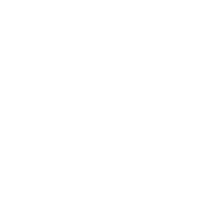
\includegraphics[max width=\textwidth]{calculations/814.png}
  \caption{Type figure caption here}
  \label{fig:814}
 \end{center}
\end{figure}
%%%
\begin{equation*}
\textit{F}_{\textit{iomin34}} \defeq 0.62 \cdot \textit{K}_{\textit{s34}} \cdot \left( \textit{F}_{\textit{i3}}+\textit{F}_{\textit{i4}} \right) = {27.3296}
\end{equation*}
%%%
\begin{equation*}
\textit{F}_{\textit{iomin56}} \defeq 0.62 \cdot \textit{K}_{\textit{s56}} \cdot \left( \textit{F}_{\textit{i5}}+\textit{F}_{\textit{i6}} \right) = {27.9868}
\end{equation*}
%%%
\begin{equation*}
\textit{F}_{\textit{iomin56}} \defeq 0.62 \cdot \textit{K}_{\textit{s78}} \cdot \left( \textit{F}_{\textit{i7}}+\textit{F}_{\textit{i8}} \right) = {33.728}
\end{equation*}
%%%
\colorbox[HTML]{000000}{Максимальная кинематическая погрешность передачи:}\newline
%%%
\begin{equation*}
\textit{F}_{\textit{iomax12}} \defeq \textit{K}_{\textit{12}} \cdot \left( \sqrt{\textit{F}_{\textit{i1}}^{2}+E_{ΣM}^{2}}+\sqrt{\textit{F}_{\textit{i2}}^{2}+E_{ΣM}^{2}} \right) = {70.9435}
\end{equation*}
%%%
\begin{figure}[h!]
 \begin{center}
  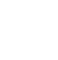
\includegraphics[max width=\textwidth]{calculations/820.png}
  \caption{Type figure caption here}
  \label{fig:820}
 \end{center}
\end{figure}
%%%
\begin{equation*}
\textit{F}_{\textit{iomax34}} \defeq \textit{K}_{\textit{34}} \cdot \left( \sqrt{\textit{F}_{\textit{i3}}^{2}+E_{ΣM}^{2}}+\sqrt{\textit{F}_{\textit{i4}}^{2}+E_{ΣM}^{2}} \right) = {70.9435}
\end{equation*}
%%%
\begin{equation*}
\textit{F}_{\textit{iomax56}} \defeq \textit{K}_{\textit{56}} \cdot \left( \sqrt{\textit{F}_{\textit{i5}}^{2}+E_{ΣM}^{2}}+\sqrt{\textit{F}_{\textit{i6}}^{2}+E_{ΣM}^{2}} \right) = {79.6403}
\end{equation*}
%%%
\begin{equation*}
\textit{F}_{\textit{iomax78}} \defeq \textit{K}_{\textit{78}} \cdot \left( \sqrt{\textit{F}_{\textit{i7}}^{2}+E_{ΣM}^{2}}+\sqrt{\textit{F}_{\textit{i8}}^{2}+E_{ΣM}^{2}} \right) = {87.3951}
\end{equation*}
%%%
\colorbox[HTML]{000000}{Максимальная кинематическая погрешность в угловых единицах:}\newline
%%%
\begin{equation*}
\textit{δφ}_{\textit{12}} \defeq 6.88 \cdot \frac{\textit{F}_{\textit{iomax12}}}{\textit{d}_{\textit{2}} \cdot 1000} = {18.7727 \cdot \frac{1}{\mathrm{m}}}
\end{equation*}
%%%
\begin{equation*}
\textit{δφ}_{\textit{56}} \defeq 6.88 \cdot \frac{\textit{F}_{\textit{iomax56}}}{\textit{d}_{\textit{6}} \cdot 1000} = {12.4529 \cdot \frac{1}{\mathrm{m}}}
\end{equation*}
%%%
\begin{figure}[h!]
 \begin{center}
  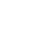
\includegraphics[max width=\textwidth]{calculations/827.png}
  \caption{Type figure caption here}
  \label{fig:827}
 \end{center}
\end{figure}
%%%
\begin{figure}[h!]
 \begin{center}
  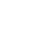
\includegraphics[max width=\textwidth]{calculations/828.png}
  \caption{Type figure caption here}
  \label{fig:828}
 \end{center}
\end{figure}
%%%
\begin{equation*}
\textit{δφ}_{\textit{34}} \defeq 6.88 \cdot \frac{\textit{F}_{\textit{iomax34}}}{\textit{d}_{\textit{4}} \cdot 1000} = {16.2697 \cdot \frac{1}{\mathrm{m}}}
\end{equation*}
%%%
\begin{equation*}
\textit{δφ}_{\textit{78}} \defeq 6.88 \cdot \frac{\textit{F}_{\textit{iomax78}}}{\textit{d}_{\textit{8}} \cdot 1000} = {9.5441 \cdot \frac{1}{\mathrm{m}}}
\end{equation*}
%%%
\begin{figure}[h!]
 \begin{center}
  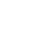
\includegraphics[max width=\textwidth]{calculations/831.png}
  \caption{Type figure caption here}
  \label{fig:831}
 \end{center}
\end{figure}
%%%
\begin{figure}[h!]
 \begin{center}
  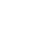
\includegraphics[max width=\textwidth]{calculations/832.png}
  \caption{Type figure caption here}
  \label{fig:832}
 \end{center}
\end{figure}
%%%
\begin{equation*}
δφ_{maxΣ} \defeq \frac{\textit{δφ}_{\textit{12}}}{\textit{i}_{\textit{34}} \cdot \textit{i}_{\textit{56}} \cdot \textit{i}_{\textit{78}}}+\frac{\textit{δφ}_{\textit{34}}}{\textit{i}_{\textit{56}} \cdot \textit{i}_{\textit{78}}}+\frac{\textit{δφ}_{\textit{56}}}{\textit{i}_{\textit{78}}}+\frac{\textit{δφ}_{\textit{78}}}{1} = {15.1339 \cdot \frac{1}{\mathrm{m}}}
\end{equation*}
%%%
\begin{figure}[h!]
 \begin{center}
  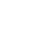
\includegraphics[max width=\textwidth]{calculations/834.png}
  \caption{Type figure caption here}
  \label{fig:834}
 \end{center}
\end{figure}
%%%
\colorbox[HTML]{000000}{18. Кинематический мертвый ход зубчатой передачи.}\newline
%%%
\colorbox[HTML]{000000}{Наименьшие дополнительные смещения исходного контура:}\newline
%%%
\begin{equation*}
\textit{E}_{\textit{HS1}} \defeq 32
\end{equation*}
%%%
\begin{equation*}
\textit{E}_{\textit{HS5}} \defeq 32
\end{equation*}
%%%
\begin{equation*}
\textit{E}_{\textit{HS2}} \defeq 38
\end{equation*}
%%%
\begin{equation*}
\textit{E}_{\textit{HS6}} \defeq 45
\end{equation*}
%%%
\begin{equation*}
\textit{E}_{\textit{HS3}} \defeq 28
\end{equation*}
%%%
\begin{equation*}
\textit{E}_{\textit{HS7}} \defeq 28
\end{equation*}
%%%
\begin{equation*}
\textit{E}_{\textit{HS4}} \defeq 38
\end{equation*}
%%%
\begin{equation*}
\textit{E}_{\textit{HS8}} \defeq 53
\end{equation*}
%%%
\colorbox[HTML]{000000}{Допуск на радиальное биение зубчатого венца:}\newline
%%%
\begin{figure}[h!]
 \begin{center}
  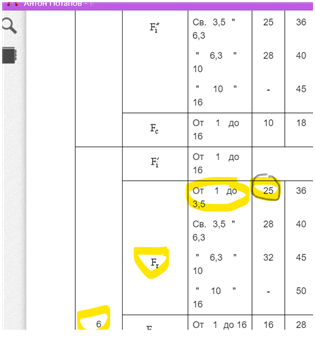
\includegraphics[max width=\textwidth]{calculations/846.png}
  \caption{Type figure caption here}
  \label{fig:846}
 \end{center}
\end{figure}
%%%
\colorbox[HTML]{000000}{Допуск на смещение исходного контура:}\newline
%%%
\begin{equation*}
T_{H} \defeq 56
\end{equation*}
%%%
\colorbox[HTML]{000000}{Гарантированный боковой зазор:}\newline
%%%
\begin{equation*}
\textit{j}_{\textit{nmin12}} \defeq 21
\end{equation*}
%%%
\begin{equation*}
\textit{j}_{\textit{nmin56}} \defeq 21
\end{equation*}
%%%
\begin{equation*}
\textit{j}_{\textit{nmin34}} \defeq 21
\end{equation*}
%%%
\begin{equation*}
\textit{j}_{\textit{nmin78}} \defeq 25
\end{equation*}
%%%
\colorbox[HTML]{000000}{Минимальный кинематический мертвый ход передачи:}\newline
%%%
\begin{equation*}
\textit{j}_{\textit{tmin12}} \defeq \frac{\textit{j}_{\textit{nmin12}}}{\cos \left( {\alpha} \right) \cdot \cos \left( {\beta} \right)} = {22.3477}
\end{equation*}
%%%
\begin{equation*}
\textit{j}_{\textit{tmin56}} \defeq \frac{\textit{j}_{\textit{nmin56}}}{\cos \left( {\alpha} \right) \cdot \cos \left( {\beta} \right)} = {22.3477}
\end{equation*}
%%%
\begin{equation*}
\textit{j}_{\textit{tmin34}} \defeq \frac{\textit{j}_{\textit{nmin34}}}{\cos \left( {\alpha} \right) \cdot \cos \left( {\beta} \right)} = {22.3477}
\end{equation*}
%%%
\begin{equation*}
\textit{j}_{\textit{tmin78}} \defeq \frac{\textit{j}_{\textit{nmin78}}}{\cos \left( {\alpha} \right) \cdot \cos \left( {\beta} \right)} = {26.6044}
\end{equation*}
%%%
\colorbox[HTML]{000000}{Предельные отклонения межосевого расстояния:}\newline
%%%
\begin{equation*}
\textit{f}_{\textit{a12}} \defeq 40
\end{equation*}
%%%
\begin{equation*}
\textit{f}_{\textit{a34}} \defeq 40
\end{equation*}
%%%
\begin{equation*}
\textit{f}_{\textit{a56}} \defeq 40
\end{equation*}
%%%
\begin{equation*}
\textit{f}_{\textit{a78}} \defeq 50
\end{equation*}
%%%
\colorbox[HTML]{000000}{Максимальный кинематический мертвый ход передачи:}\newline
%%%
\begin{equation*}
\textit{j}_{\textit{tmax12}} \defeq 0.7 \cdot \left( \textit{E}_{\textit{HS1}}+\textit{E}_{\textit{HS2}} \right)+\sqrt{0.5 \cdot \left( T_{H}^{2}+T_{H}^{2} \right)+2 \cdot \textit{f}_{\textit{a12}}^{2}+G_{r}^{2}+G_{r}^{2}} = {133.4748}
\end{equation*}
%%%
\begin{equation*}
\textit{j}_{\textit{tmax34}} \defeq 0.7 \cdot \left( \textit{E}_{\textit{HS3}}+\textit{E}_{\textit{HS4}} \right)+\sqrt{0.5 \cdot \left( T_{H}^{2}+T_{H}^{2} \right)+2 \cdot \textit{f}_{\textit{a34}}^{2}+G_{r}^{2}+G_{r}^{2}} = {130.6748}
\end{equation*}
%%%
\begin{equation*}
\textit{j}_{\textit{tmax56}} \defeq 0.7 \cdot \left( \textit{E}_{\textit{HS1}}+\textit{E}_{\textit{HS2}} \right)+\sqrt{0.5 \cdot \left( T_{H}^{2}+T_{H}^{2} \right)+2 \cdot \textit{f}_{\textit{a56}}^{2}+G_{r}^{2}+G_{r}^{2}} = {133.4748}
\end{equation*}
%%%
\begin{equation*}
\textit{j}_{\textit{tmax78}} \defeq 0.7 \cdot \left( \textit{E}_{\textit{HS1}}+\textit{E}_{\textit{HS2}} \right)+\sqrt{0.5 \cdot \left( T_{H}^{2}+T_{H}^{2} \right)+2 \cdot \textit{f}_{\textit{a78}}^{2}+G_{r}^{2}+G_{r}^{2}} = {143.5304}
\end{equation*}
%%%
\colorbox[HTML]{000000}{Минимальное и максимальное значение мертвого хода передачи в угловых единицах:}\newline
%%%
\colorbox[HTML]{000000}{(Домножил знаменатель на 1000 для получения правильной размерности угл. мин)}\newline
%%%
\begin{equation*}
\textit{j}_{\textit{φmin12}} \defeq 7.32 \cdot \frac{\textit{j}_{\textit{tmin12}}}{\textit{d}_{\textit{2}} \cdot 1000} = {6.2917 \cdot \frac{1}{\mathrm{m}}}
\end{equation*}
%%%
\begin{figure}[h!]
 \begin{center}
  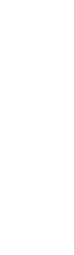
\includegraphics[max width=\textwidth]{calculations/872.png}
  \caption{Type figure caption here}
  \label{fig:872}
 \end{center}
\end{figure}
%%%
\begin{equation*}
\textit{j}_{\textit{φmin34}} \defeq 7.32 \cdot \frac{\textit{j}_{\textit{tmin34}}}{\textit{d}_{\textit{4}} \cdot 1000} = {5.4528 \cdot \frac{1}{\mathrm{m}}}
\end{equation*}
%%%
\begin{figure}[h!]
 \begin{center}
  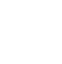
\includegraphics[max width=\textwidth]{calculations/874.png}
  \caption{Type figure caption here}
  \label{fig:874}
 \end{center}
\end{figure}
%%%
\begin{equation*}
\textit{j}_{\textit{φmin56}} \defeq 7.32 \cdot \frac{\textit{j}_{\textit{tmin56}}}{\textit{d}_{\textit{6}} \cdot 1000} = {3.7179 \cdot \frac{1}{\mathrm{m}}}
\end{equation*}
%%%
\begin{figure}[h!]
 \begin{center}
  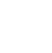
\includegraphics[max width=\textwidth]{calculations/876.png}
  \caption{Type figure caption here}
  \label{fig:876}
 \end{center}
\end{figure}
%%%
\begin{equation*}
\textit{j}_{\textit{φmin78}} \defeq 7.32 \cdot \frac{\textit{j}_{\textit{tmin78}}}{\textit{d}_{\textit{8}} \cdot 1000} = {3.0912 \cdot \frac{1}{\mathrm{m}}}
\end{equation*}
%%%
\begin{figure}[h!]
 \begin{center}
  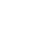
\includegraphics[max width=\textwidth]{calculations/878.png}
  \caption{Type figure caption here}
  \label{fig:878}
 \end{center}
\end{figure}
%%%
\colorbox[HTML]{000000}{(Домножил знаменатель на 1000 для получения правильной размерности угл. мин)}\newline
%%%
\begin{equation*}
\textit{j}_{\textit{φmax12}} \defeq 7.32 \cdot \frac{\textit{j}_{\textit{tmax12}}}{\textit{d}_{\textit{2}} \cdot 1000} = {37.5783 \cdot \frac{1}{\mathrm{m}}}
\end{equation*}
%%%
\begin{figure}[h!]
 \begin{center}
  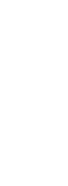
\includegraphics[max width=\textwidth]{calculations/881.png}
  \caption{Type figure caption here}
  \label{fig:881}
 \end{center}
\end{figure}
%%%
\begin{equation*}
\textit{j}_{\textit{φmax34}} \defeq 7.32 \cdot \frac{\textit{j}_{\textit{tmax34}}}{\textit{d}_{\textit{4}} \cdot 1000} = {31.8847 \cdot \frac{1}{\mathrm{m}}}
\end{equation*}
%%%
\begin{figure}[h!]
 \begin{center}
  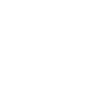
\includegraphics[max width=\textwidth]{calculations/883.png}
  \caption{Type figure caption here}
  \label{fig:883}
 \end{center}
\end{figure}
%%%
\begin{figure}[h!]
 \begin{center}
  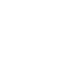
\includegraphics[max width=\textwidth]{calculations/884.png}
  \caption{Type figure caption here}
  \label{fig:884}
 \end{center}
\end{figure}
%%%
\begin{equation*}
\textit{j}_{\textit{φmax56}} \defeq 7.32 \cdot \frac{\textit{j}_{\textit{tmax56}}}{\textit{d}_{\textit{6}} \cdot 1000} = {22.2054 \cdot \frac{1}{\mathrm{m}}}
\end{equation*}
%%%
\begin{figure}[h!]
 \begin{center}
  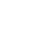
\includegraphics[max width=\textwidth]{calculations/886.png}
  \caption{Type figure caption here}
  \label{fig:886}
 \end{center}
\end{figure}
%%%
\begin{equation*}
\textit{j}_{\textit{φmax78}} \defeq 7.32 \cdot \frac{\textit{j}_{\textit{tmax78}}}{\textit{d}_{\textit{8}} \cdot 1000} = {16.6769 \cdot \frac{1}{\mathrm{m}}}
\end{equation*}
%%%
\begin{figure}[h!]
 \begin{center}
  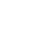
\includegraphics[max width=\textwidth]{calculations/888.png}
  \caption{Type figure caption here}
  \label{fig:888}
 \end{center}
\end{figure}
%%%
\colorbox[HTML]{000000}{Кинематический мертвый ход многозвенного механизма, приведенный к выходному звену:}\newline
%%%
\begin{equation*}
j_{φmaxΣ} \defeq \frac{\textit{j}_{\textit{φmax12}}}{\textit{i}_{\textit{34}} \cdot \textit{i}_{\textit{56}} \cdot \textit{i}_{\textit{78}}}+\frac{\textit{j}_{\textit{φmax34}}}{\textit{i}_{\textit{56}} \cdot \textit{i}_{\textit{78}}}+\frac{\textit{j}_{\textit{φmax56}}}{\textit{i}_{\textit{78}}}+\frac{\textit{j}_{\textit{φmax78}}}{1} = {27.1118 \cdot \frac{1}{\mathrm{m}}}
\end{equation*}
%%%
\begin{figure}[h!]
 \begin{center}
  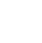
\includegraphics[max width=\textwidth]{calculations/891.png}
  \caption{Type figure caption here}
  \label{fig:891}
 \end{center}
\end{figure}
%%%
\colorbox[HTML]{000000}{\textbf{19. Расчет упругого мертвого хода:}}\newline
%%%
\colorbox[HTML]{000000}{Полярные моменты инерции валов:}\newline
%%%
\begin{equation*}
J_{pI} \defeq {\pi} \cdot \frac{d_{I}^{4}}{32} = {25.1327}
\end{equation*}
%%%
\begin{equation*}
J_{pII} \defeq {\pi} \cdot \frac{d_{II}^{4}}{32} = {61.3592}
\end{equation*}
%%%
\begin{equation*}
J_{pIII} \defeq {\pi} \cdot \frac{d_{III}^{4}}{32} = {61.3592}
\end{equation*}
%%%
\begin{equation*}
J_{pIV} \defeq {\pi} \cdot \frac{d_{IV}^{4}}{32} = {61.3592}
\end{equation*}
%%%
\begin{equation*}
J_{pV} \defeq {\pi} \cdot \frac{d_{V}^{4}}{32} = {127.2345}
\end{equation*}
%%%
\colorbox[HTML]{000000}{Длины участков валов, на которые действует крутящий момент:}\newline
%%%
\begin{equation*}
\textit{l}_{\textit{1}} \defeq 4
\end{equation*}
%%%
\begin{equation*}
\textit{l}_{\textit{2}} \defeq 20.5
\end{equation*}
%%%
\begin{equation*}
\textit{l}_{\textit{3}} \defeq 20.5
\end{equation*}
%%%
\begin{equation*}
\textit{l}_{\textit{4}} \defeq 37.5
\end{equation*}
%%%
\begin{equation*}
\textit{l}_{\textit{5}} \defeq 39.2
\end{equation*}
%%%
\colorbox[HTML]{000000}{Деформации кручения валов:}\newline
%%%
\begin{equation*}
j_{φymaxI} \defeq \frac{10800 \cdot M_{I} \cdot \textit{l}_{\textit{1}}}{{\pi} \cdot J_{pI} \cdot G} = {8.7849 \cdot 10^{ \operatorname{-} 11} \: \mathrm{m}^{3}}
\end{equation*}
%%%
\begin{figure}[h!]
 \begin{center}
  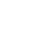
\includegraphics[max width=\textwidth]{calculations/907.png}
  \caption{Type figure caption here}
  \label{fig:907}
 \end{center}
\end{figure}
%%%
\begin{equation*}
j_{φymaxII} \defeq \frac{10800 \cdot M_{II} \cdot \textit{l}_{\textit{2}}}{{\pi} \cdot J_{pII} \cdot G} = {2.8022 \cdot 10^{ \operatorname{-} 10} \: \mathrm{m}^{3}}
\end{equation*}
%%%
\begin{figure}[h!]
 \begin{center}
  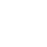
\includegraphics[max width=\textwidth]{calculations/909.png}
  \caption{Type figure caption here}
  \label{fig:909}
 \end{center}
\end{figure}
%%%
\begin{equation*}
j_{φymaxIII} \defeq \frac{10800 \cdot M_{III} \cdot \textit{l}_{\textit{3}}}{{\pi} \cdot J_{pIII} \cdot G} = {4.9949 \cdot 10^{ \operatorname{-} 10} \: \mathrm{m}^{3}}
\end{equation*}
%%%
\begin{figure}[h!]
 \begin{center}
  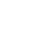
\includegraphics[max width=\textwidth]{calculations/911.png}
  \caption{Type figure caption here}
  \label{fig:911}
 \end{center}
\end{figure}
%%%
\begin{equation*}
j_{φymaxIV} \defeq \frac{10800 \cdot M_{IV} \cdot \textit{l}_{\textit{4}}}{{\pi} \cdot J_{pIV} \cdot G} = {2.4266 \cdot 10^{ \operatorname{-} 9} \: \mathrm{m}^{3}}
\end{equation*}
%%%
\begin{figure}[h!]
 \begin{center}
  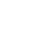
\includegraphics[max width=\textwidth]{calculations/913.png}
  \caption{Type figure caption here}
  \label{fig:913}
 \end{center}
\end{figure}
%%%
\begin{equation*}
j_{φymaxV} \defeq \frac{10800 \cdot M_{V} \cdot \textit{l}_{\textit{5}}}{{\pi} \cdot J_{pV} \cdot G} = {4.7 \cdot 10^{ \operatorname{-} 9} \: \mathrm{m}^{3}}
\end{equation*}
%%%
\begin{figure}[h!]
 \begin{center}
  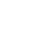
\includegraphics[max width=\textwidth]{calculations/915.png}
  \caption{Type figure caption here}
  \label{fig:915}
 \end{center}
\end{figure}
%%%
\begin{equation*}
j_{φymaxΣ} \defeq \frac{j_{φymaxI}}{\textit{i}_{\textit{12}} \cdot \textit{i}_{\textit{34}} \cdot \textit{i}_{\textit{56}} \cdot \textit{i}_{\textit{78}}}+\frac{j_{φymaxII}}{\textit{i}_{\textit{34}} \cdot \textit{i}_{\textit{56}} \cdot \textit{i}_{\textit{78}}}+\frac{j_{φymaxIII}}{\textit{i}_{\textit{56}} \cdot \textit{i}_{\textit{78}}}+\frac{j_{φymaxIV}}{\textit{i}_{\textit{78}}}+\frac{j_{φymaxV}}{1} = {5.3788 \cdot 10^{ \operatorname{-} 9} \: \mathrm{m}^{3}}
\end{equation*}
%%%
\begin{figure}[h!]
 \begin{center}
  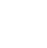
\includegraphics[max width=\textwidth]{calculations/917.png}
  \caption{Type figure caption here}
  \label{fig:917}
 \end{center}
\end{figure}
%%%
\end{document}
